%\documentclass[acmtog,anonymous,timestamp,review]{acmart}
\documentclass[acmtog]{acmart}

%\usepackage{titlesec}
%\titleformat*{\paragraph}{\large\bfseries}

%\usepackage[T1]{fontenc}
%\usepackage{lmodern}
\usepackage{booktabs} % For formal tables
\usepackage{comment}
\usepackage[textfont=normalfont,labelfont=bf]{caption}
\usepackage{subcaption}
\usepackage{overpic,bm}
\usepackage{multirow}

\acmPrice{15.00}
\acmSubmissionID{283}

% The next six lines come directly from the completed rights form.
% You MUST replace them with the lines specific to your accepted work.
%\copyrightyear{2018}
%\acmYear{2018}
%\setcopyright{rightsretained}
%\acmConference{Conference Name}{Conference Date and Year}{Conference Location}
%\acmDOI{10.1145/8888888.7777777}
%\acmISBN{978-1-4503-1234-5/17/07}

\setcopyright{acmcopyright}
\acmJournal{TOG}
\acmYear{2018}
\acmVolume{37}
\acmNumber{6}
\acmArticle{279}
\acmMonth{11} 
\acmDOI{10.1145/3272127.3275053}

% Use the "authoryear" citation style, and make sure citations are in [square brackets].
\citestyle{acmauthoryear}
\setcitestyle{square}

% A useful command for controlling the number of authors per row.
% The default value of "authorsperrow" is 2.
\settopmatter{authorsperrow=4}

% end of preamble.

\iffalse
%\iftrue
\newcommand{\sz}[1]{{\color{blue}#1}}
\newcommand{\szrem}[1]{{\color{blue}[SZ: #1]}}
\newcommand{\mhrem}[1]{{\color{red}[MH: #1]}}
\newcommand{\todo}[1]{\marginpar{\Large {\color{red} $\spadesuit$}} {\bf \color{red} [Todo: #1]}}
\else
\newcommand{\sz}[1]{#1}
\newcommand{\szrem}[1]{}
\newcommand{\todo}[1]{}
\fi

\newcommand{\E}{\mathrm{e}}
\newcommand{\bd}{\bm{d}}
\newcommand{\bx}{\bm{x}}
\newcommand{\by}{\bm{y}}
\newcommand{\bp}{\bm{p}}
\newcommand{\bq}{\bm{q}}
\newcommand{\br}{\bm{r}}
\newcommand{\bn}{\bm{n}}
\newcommand{\bb}{\bm{b}}
\newcommand{\bt}{\bm{t}}
\newcommand{\calt}{\mathcal{T}}
\newcommand{\bom}{\bm{\omega}}
\newcommand{\bal}{\bm{\alpha}}
\newcommand{\bsm}{\bm{m}}
\newcommand{\bh}{\bm{h}}
\newcommand{\BO}{\mathbb{B}_0}
\newcommand{\intd}{\,\mathrm{d}}
\newcommand{\Real}{\mathbb{R}}
\newcommand{\pr}{\mathbb{P}}
\newcommand{\ind}{\mathbb{I}}

\newcommand\relphantom[1]{\mathrel{\phantom{#1}}}
\newcommand{\argmin}{\operatornamewithlimits{argmin}}

\newcommand{\omegain}{\bm{\omega}_i}
\newcommand{\omegaout}{\bm{\omega}_o}
\newcommand{\Sph}{{\mathcal S^2}}
\newcommand{\dd}{\mbox{d}}
\newcommand{\rev}{\mathrm{rev}}

\newcommand{\myparagraph}[1]{\vspace{\baselineskip} \noindent {\bf #1.}}


% Alter some LaTeX defaults for better treatment of figures:
% See p.105 of "TeX Unbound" for suggested values.
% See pp. 199-200 of Lamport's "LaTeX" book for details.
%   General parameters, for ALL pages:
\renewcommand{\topfraction}{0.9}	% max fraction of floats at top
\renewcommand{\bottomfraction}{0.8}	% max fraction of floats at bottom
%   Parameters for TEXT pages (not float pages):
\setcounter{topnumber}{2}
\setcounter{bottomnumber}{2}
\setcounter{totalnumber}{4}     % 2 may work better
\setcounter{dbltopnumber}{2}    % for 2-column pages
\renewcommand{\dbltopfraction}{0.99}	% fit big float above 2-col. text
\renewcommand{\textfraction}{0.01}	% allow minimal text w. figs
%   Parameters for FLOAT pages (not text pages):
\renewcommand{\floatpagefraction}{0.7}	% require fuller float pages
% N.B.: floatpagefraction MUST be less than topfraction !!
\renewcommand{\dblfloatpagefraction}{0.7}	% require fuller float pages


\begin{document}

% Title. 
% If your title is long, consider \title[short title]{full title} - "short title" will be used for running heads.
\title{Position-Free Monte Carlo Simulation for Arbitrary Layered BSDFs}

% Authors.
\author{Yu Guo}
\affiliation{%
  %\department{Department of Computer Science}
  \institution{University of California, Irvine}}
\email{guo.yu@uci.edu}

\author{Milo\v{s} Ha\v{s}an}
\affiliation{%
  \institution{Autodesk}}
\email{miloshasan@gmail.com}

\author{Shuang Zhao}
\affiliation{%
  \institution{University of California, Irvine}}
\email{shz@ics.uci.edu}

% This command defines the author string for running heads.
\renewcommand{\shortauthors}{Guo, Ha\v{s}an, and Zhao}

\begin{abstract}
Real-world materials are often layered: metallic paints, biological tissues, and many more. Variation in the interface and volumetric scattering properties of the layers leads to a rich diversity of material appearances from anisotropic highlights to complex textures and relief patterns. However, simulating light-layer interactions is a challenging problem. Past analytical or numerical solutions either introduce several approximations and limitations, or rely on expensive operations on discretized BSDFs, preventing the ability to freely vary the layer properties spatially. We introduce a new unbiased layered BSDF model based on Monte Carlo simulation, whose only assumption is the layer assumption itself. Our novel position-free path formulation is fundamentally more powerful at constructing light transport paths than generic light transport algorithms applied to the special case of flat layers, since it is based on a product of solid angle instead of area measures, so does not contain the high-variance geometry terms needed in the standard formulation. We introduce two techniques for sampling the position-free path integral, a forward path tracer with next-event estimation and a full bidirectional estimator. We show a number of examples, featuring multiple layers with surface and volumetric scattering, surface and phase function anisotropy, and spatial variation in all parameters.
\end{abstract}


%CCS
\begin{CCSXML}
<ccs2012>
<concept>
<concept_id>10010147.10010371.10010372</concept_id>
<concept_desc>Computing methodologies~Rendering</concept_desc>
<concept_significance>500</concept_significance>
</concept>
<concept>
<concept_id>10010147.10010371.10010372.10010374</concept_id>
<concept_desc>Computing methodologies~Ray tracing</concept_desc>
<concept_significance>500</concept_significance>
</concept>
</ccs2012>
\end{CCSXML}

%\ccsdesc[500]{Computing methodologies~Rendering}
%\ccsdesc[500]{Computing methodologies~Ray tracing}

%keywords
\keywords{BSDF, layered materials, Monte Carlo integration}

% A "teaser" figure, centered below the title and authors and above the body of the work.
\begin{teaserfigure}
	\centering
	\newlength{\imgHeight}
	\setlength{\imgHeight}{2.3in}
	\addtolength{\tabcolsep}{-3.5pt}
	\begin{tabular}{ccccc}
		\begin{overpic}[height=\imgHeight]{img/teaser/teaser.jpg}
			\put(2,3){\bfseries \color{white} \Large (a)}
		\end{overpic}
		&
		\begin{overpic}[height=\imgHeight]{img/teaser/green.jpg}
			\put(2,3){\bfseries \color{white} \Large (b1)}
		\end{overpic}
		&
		\begin{overpic}[height=\imgHeight]{img/teaser/yellow.jpg}
			\put(2,3){\bfseries \color{white} \Large (c1)}
		\end{overpic}
		&
		\begin{overpic}[height=\imgHeight]{img/teaser/blue.jpg}
			\put(2,3){\bfseries \color{white} \Large (d1)}
		\end{overpic}
		&
		\begin{overpic}[height=\imgHeight]{img/teaser/magenta.jpg}
			\put(2,3){\bfseries \color{white} \Large (e1)}
		\end{overpic}
	\end{tabular}
	\\[3pt]
	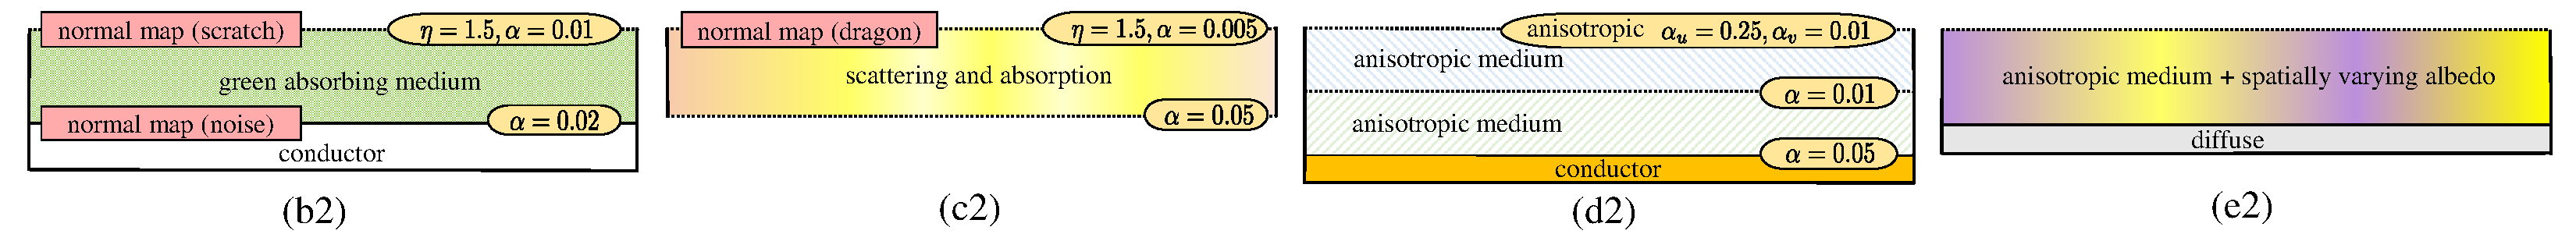
\includegraphics[width=\textwidth]{img/teaser/illustration.pdf}
	\caption{\label{fig:teaser}
		We introduce a new BSDF model leveraging an efficient Monte Carlo simulation algorithm applied locally to layered geometries.
		Our model enjoys the flexibility of using arbitrary layer interfaces and internal media and is capable of reproducing a wide variety of appearances.
		This example contains three vases on a tablecloth, all described using our BSDF model (see the insets for layer configurations).
	}
\end{teaserfigure}


% Processes all of the front-end information and starts the body of the work.
\maketitle

\section{Introduction}
\label{sec:intro}

Physically-based shading models have become mature and commonplace in recent years across a number of rendering applications, within entertainment, architecture, and industrial design. However, we are seeing constant progress in the area of material reflection and scattering models, aiming to achieve higher physical realism and to enable more effective material content creation.

% 1. Motivation: the importance of layered materials
%
Many real world materials are comprised of thin layers with varying compositions. For example, metallic paint is a dielectric coating covering a metallic substrate composed of randomly oriented aluminum flakes; the absorption and scattering properties of the dielectric layer give the material its color and modify its directional scattering properties as well.
%Many biological materials (e.g. plant leaves) are also layered, and their appearance is a complex combination of the absorption properties, scattering phase function, air-material interface roughness, and thickness variation.
Different characteristics of such interfaces and volumetric scattering properties can produce richly diverse material appearances from anisotropic highlights to complex textures. Furthermore, detailed layer thickness variations, scratches and bumps on the layer interfaces give these materials additional richness. Accurately understanding and simulating these interactions is therefore key to further progress in the rendering of materials.

% 2. Challenge: it is hard to simulate light-layer interactions
%
However, explicitly simulating light-layer interactions by modeling the full geometry of these layers would be very expensive and cumbersome.
The complex and spatially varying interface and internal microgeometries are much too costly to describe and simulate using standard 3D scene modeling tools such as triangle meshes and volumetric grids.
%Furthermore, due to the presence of multiple refractive interfaces, it can be very challenging to correctly construct light transport paths that connect light scattering locations to light sources, a key opration in most practical Monte Carlo rendering systems. Cheap approximations to these light transport problems (e.g. ignoring refraction, or composing layers using simple blending) are not sufficient to achieve true realism.

% 3. A brief recap on existing methods
%
A few techniques have been developed to address this problem. Weidlich and Wilkie~\shortcite{Weidlich:2007:ALM} construct a simple and flexible analytical model. However, significant approximations are necessary; interface roughness is not fully handled for transmission, and no volumetric scattering is supported. The work of Belcour~\shortcite{Belcour2018} recently introduced a more advanced approach based on tracking low-order moments of the BSDF lobes; however, it still introduces some approximations and limitations. On the other hand, Jakob et al.~\shortcite{Jakob:2014:CFR} (with a recent follow-up \cite{Zeltner2018}) introduce a solution that is very accurate, but expensive: it represents BSDFs as discretized datasets and relies on expensive Fourier-domain operations on these to implement layer composition and thickness adjustment. This makes free spatial variation of the layer properties prohibitively expensive: a significant limitation in practice.

%These methods, like ours, utilize microfacet models (e.g., \cite{Walter:2007:MMR}) to describe the interface reflection and transmission properties.
%while others only handle interfacial interactions and ignore volumetric scatterings (e.g., \cite{guo2017rendering}).

% 4. Overview of our approach and our contributions
%
In this paper, we introduce a new layered BSDF model without the above limitations. Our model provides an accurate, unbiased solution; to our knowledge, it is the only such model.
Unlike previous work, we do not attempt to derive an analytic model for the BSDF lobe shapes. Instead, inside the evaluation and sampling routines of the layered BSDF, we run a Monte Carlo simulation of light transport within flat slabs.
%This is substantially faster than explicitly constructing the layer geometry, because no expensive scene ray tracing is required.
%Our model computes an accurate solution of the layered light transport problem.
%It is based on physical interface and volume scattering models, conserves energy and is reciprocal when possible. It can also be easily integrated into standard Monte Carlo rendering systems.
This requires no precomputation and thus can efficiently handle spatially varying appearances. It also supports the full range of editability of the layer properties, both interface and volumetric, and allows anisotropy in both interface BSDFs and phase functions. In fact, the only limiting assumption of our model is the layer assumption itself.

Our solution is fundamentally more powerful at constructing light transport paths than generic transport algorithms (e.g standard path tracing, bidirectional or Metropolis transport); see Figure \ref{fig:validation1}. We introduce a modified path integral framework for light transport in flat slabs, superior to the standard path formulation in this setting. Because it is based on a product of solid angle instead of area measures, it does not contain the high-variance geometry terms needed in standard algorithms. We introduce two simulation techniques within this formulation: the first is analogous to a forward path tracer with next event estimation through layer boundaries and multiple importance sampling; the second is a fully bidirectional estimator. We show the capabilities of this solution on a number of examples, featuring multiple layers with surface and volumetric scattering. Our examples show spatial variation in all parameters: surface BSDF, volume and phase function parameters, layer thickness and surface normal.


%
\section{Related Work}
\label{sec:related}

\begin{figure*}[t]
	\centering
	\addtolength{\tabcolsep}{-4pt}
	\begin{tabular}{cccccc}
		\begin{overpic}[width=0.16\textwidth]{img/validations/compare1/plane_fullsim_ref_3_2h.jpg} 
			%\put(2,3){\bfseries \color{white} \Large } 
		\end{overpic} &
		\begin{overpic}[width=0.16\textwidth]{img/validations/compare1/plane_10s_pt_98spp.jpg} 
			\put(2,3){\bfseries \color{white} 98 spp} 
		\end{overpic} &
		\begin{overpic}[width=0.16\textwidth]{img/validations/compare1/plane_10s_bdpt_35spp.jpg} 
			\put(2,3){\bfseries \color{white} 35 spp} 
		\end{overpic} &
		\begin{overpic}[width=0.16\textwidth]{img/validations/compare1/plane_10s_mlt_280spp.jpg}
			\put(2,3){\bfseries \color{white} 280 spp} 
		\end{overpic} &
		\begin{overpic}[width=0.16\textwidth]{img/validations/compare1/plane_10s_uni_56spp.jpg} 
			\put(2,3){\bfseries \color{white} 56 spp} 
		\end{overpic} &
		\begin{overpic}[width=0.16\textwidth]{img/validations/compare1/plane_10s_bi_26spp.jpg} 
			\put(2,3){\bfseries \color{white} 26 spp} 
		\end{overpic}
		\\
		\begin{overpic}[width=0.16\textwidth]{img/validations/compare1/plane_fullsim_ref_4_8h.jpg} 
			%\put(2,3){\bfseries \color{white} \Large } 
		\end{overpic} &
		\begin{overpic}[width=0.16\textwidth]{img/validations/compare1/plane_10s_pt_60spp.jpg} 
			\put(2,3){\bfseries \color{white} 60 spp} 
		\end{overpic} &
		\begin{overpic}[width=0.16\textwidth]{img/validations/compare1/plane_10s_bdpt_25spp.jpg} 
			\put(2,3){\bfseries \color{white} 25 spp} 
		\end{overpic} &
		\begin{overpic}[width=0.16\textwidth]{img/validations/compare1/plane_10s_mlt_80spp.jpg} 
			\put(2,3){\bfseries \color{white} 80 spp} 
		\end{overpic} &
		\begin{overpic}[width=0.16\textwidth]{img/validations/compare1/plane_10s_uni_15spp.jpg} 
			\put(2,3){\bfseries \color{white} 15 spp} 
		\end{overpic} &
		\begin{overpic}[width=0.16\textwidth]{img/validations/compare1/plane_10s_bi_19spp.jpg} 
			\put(2,3){\bfseries \color{white} 19 spp} 
		\end{overpic}
		\\
		%
		Reference &
		Standard PT &
		Standard BDPT &
		Standard MLT &
		Our unidirectional &
		Our bidirectional
	\end{tabular}
	\caption{\label{fig:validation1}
		\textbf{Equal-time comparisons} of our unidirectional and bidirectional approach to standard transport algorithms, on a simple flat layered configuration lit by a small area light. 
		\sz{For standard PT, BDPT and MLT, results are all generated using 3D tracing by applying these algorithms in a simple 3D scene containing a very large slab with flat interfaces.} 
		%Again, performance is dominated by shading computation, as the scene is trivial.
		\textbf{Top}: A single slab with Henyey-Greenstein scattering between two interfaces, where our estimators perform similarly, but both significantly outperform path tracing, bidirectional and Metropolis transport. \textbf{Bottom}: A more complex configuration with two slabs and three interfaces; both media are using an anisotropic microflake phase function \cite{Jakob:2010:RTF}. Our bidirectional estimator is a clear winner in this case.
		\sz{The references are generated using standard PT with 100K spp, and all the other images are rendered in 10 seconds.}
	}
\end{figure*}


\subsection{Discretized layered BSDFs}
%\myparagraph{Discretized layered BSDFs}
Previously, a number of BSDF models have been proposed to describe layers with various assumptions on the interface and subsurface scattering.

An early analytical model by Hanrahan and Krueger \shortcite{Hanrahan1993} already supported multiple layers, but only single scattering, and without supporting arbitrary BSDFs at interfaces. They also proposed to add multiple scattering by Monte Carlo simulation, but their simulation approach only considers volume scattering events (as opposed to a combination of volume and rough interface events). Furthermore, it uses binning on the outgoing direction, as opposed to an efficient BSDF evaluation method for a given outgoing direction, which is provided by our approach.

A model by Stam \shortcite{Stam2001} introduces a solution for rendering skin as a layered material consisting of rough dielectric interfaces bounding a volumetric scattering slab. The solution is based on discretization of the BSDF into a directional basis, on which the light transport problem is solved. The model introduced by Jakob~et~al.~\shortcite{Jakob:2014:CFR} can be seen as a significant extension of Stam's discretization approach, working in the Fourier domain. It handles arbitrary layer stacks, supporting subsurface scattering within thin layers using the adding-doubling method, in addition to microfacet rough interfaces. The work of Zeltner extends this approach to anisotropic surface reflectance \shortcite{Zeltner2018}. These models are highly accurate and efficient to render with, once the discretized BSDF has been constructed. However, as the BSDF construction in the discretized basis is relatively expensive, they are best suited for homogeneous BSDFs. A small number of such BSDFs can be spatially blended with varying weights, but this has strict limitations, compared to our support for arbitrary spatial texturing of all parameters.

\subsection{Analytic layered BSDFs}
%\myparagraph{Approximate layered BSDFs}
The model by Weidlich and Wilkie \shortcite{Weidlich:2007:ALM} takes a different approach. They focus on layers where subsurface scattering is absent (though absorption is allowed), by analytically combining microfacet BSDFs from the interfaces into a single, potentially multi-lobe, microfacet-like BSDF. There are significant approximations in this approach, carefully chosen so that integration (Monte Carlo or otherwise) is never required within a single BSDF query. This makes the model fast and flexible. Another recent model \cite{guo2017rendering} also takes the approach of avoiding Monte Carlo integration during queries, by introducing extended normal distribution functions (ENDFs), analogous to microfacet NDFs but capturing multiple reflection or scattering events. In the most recent work, Belcour \shortcite{Belcour2018} introduced an approach based on tracking low-order moments of the BSDF lobes. This is a very fast and practical solution, but still introduces some approximations and limitations (e.g. no surface or volume anisotropy). In contrast, our method offers unbiased accuracy and even more flexibility, at the cost of some additional computation and variance. \sz{Several previous techniques model light scattering in layered materials like human skin~\cite{Donner:2008:LHR}, but these are focused on lateral light spreading in BSSRDFs, and are orthogonal to our focus on the directional properties of BSDF models.}

\subsection{Microfacet models for interfaces}
%\myparagraph{Microfacet models for interfaces}
BSDF models based on the microfacet theory are commonly used in computer graphics to capture how light reflects and refracts when interacting with specular surfaces with rough microstructure. The model by Walter~et~al.~\shortcite{Walter:2007:MMR} extends the microfacet model of Cook and Torrance~\shortcite{Cook:1982:RMC} to handle light reflection and transmittance through rough dielectric interfaces, and is currently seen as standard in physically-based rendering. We use this model to describe our layer interfaces.

The microfacet model recently developed by Heitz~et~al.~\shortcite{Heitz:2016:MMB} is capable of capturing interreflections between the facets and better conserves energy. Sch\"ussler \shortcite{Schussler2017} introduced a solution to the energy loss common in normal mapping techniques, caused by a mismatch between the shading and geometric normal. These models (or any future improved microfacet models) could be combined with our approach.

\subsection{Capability comparison}
%\myparagraph{Capability comparison}
In Figure \ref{fig:compare-previous}, we compare the capabilities of our approach to recent work \cite{Zeltner2018,Belcour2018}. We consider three features supported by our approach: surface anisotropy, spatial variation, and volumetric medium anisotropy. Only one of these is supported in the compared systems: spatial variation in Belcour's approach and surface anisotropy in Zeltner's.

\begin{figure}[t]
	\addtolength{\tabcolsep}{-3pt}
	\begin{tabular}{ccc}
		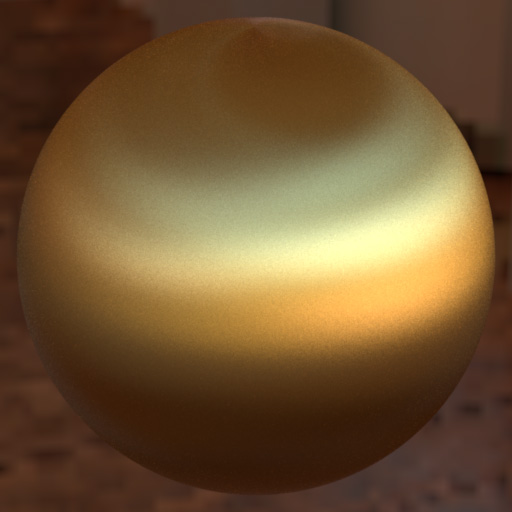
\includegraphics[width=0.315\columnwidth]{validations/compare2/aniso_comb_hor_hor_512spp_17min.jpg} &
		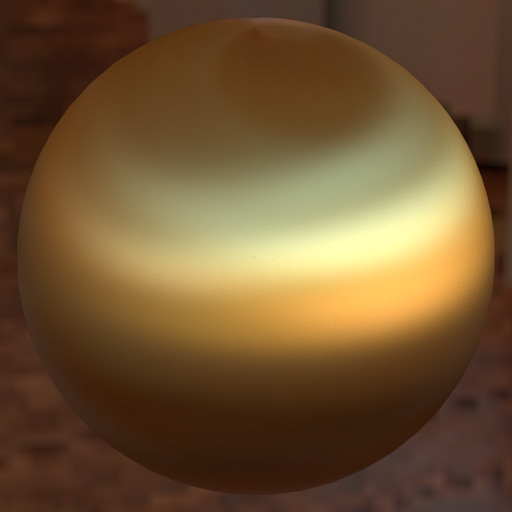
\includegraphics[width=0.315\columnwidth]{validations/compare2/aniso_comb_hor_hor_wenzel.jpg} &
		
\includegraphics[width=0.315\columnwidth]{validations/compare2/na.pdf} \\
		
		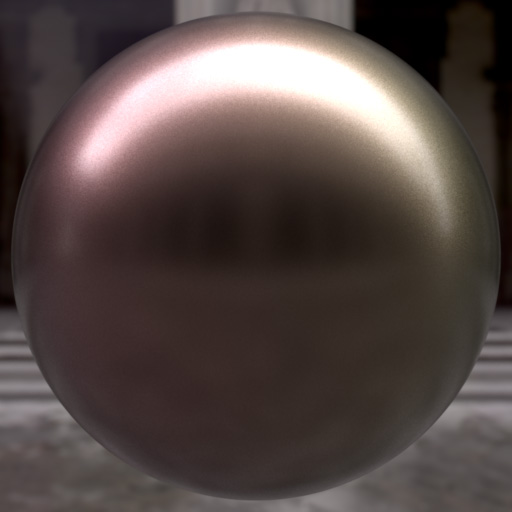
\includegraphics[width=0.315\columnwidth]{validations/compare2/sphere_layered_1024spp_37min.jpg} &
		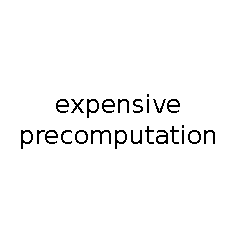
\includegraphics[width=0.315\columnwidth]{validations/compare2/na2.pdf} &
		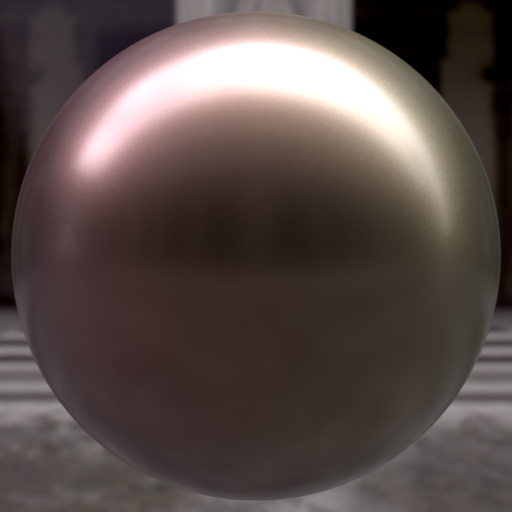
\includegraphics[width=0.315\columnwidth]{validations/compare2/sphere_laurent_1024spp_1_5min.jpg} \\
		
		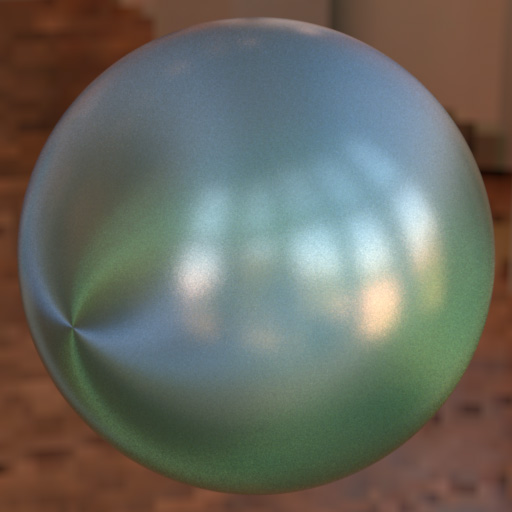
\includegraphics[width=0.315\columnwidth]{validations/compare2/sphere_1024spp_60min.jpg} &
		
\includegraphics[width=0.315\columnwidth]{validations/compare2/na.pdf} &
		
\includegraphics[width=0.315\columnwidth]{validations/compare2/na.pdf} \\
		
		Ours &
		[Zeltner 2018] &
		\cite{Belcour2018}
	\end{tabular}
	%
	\caption{\label{fig:compare-previous}
		\textbf{Comparison to previous work.} The \textbf{top row} shows an example with anisotropic surface reflectance, where our solution closely matches Zeltner's, but Belcour's approach does not support anisotropy. The \textbf{middle row} shows an example with spatial variation in the parameters; here our method closely matches Belcour's, but Zeltner's approach does not naturally support spatial variation. The \textbf{bottom row} shows a two-layer configuration with anisotropic microflake phase functions, which is only supported by our method.
	}
\end{figure}


%\sz{
%\myparagraph{Specialized models}
%Previously, a few specialized techniques have been developed to model light scattering in materials like human skin~\cite{Donner:2008:LHR} and clouds~\cite{bouthors2006real,sekiguchi2017simple}.
%These methods are largely orthogonal to this work as they focus on light transport problems with very different settings.
%}


%
\section{Background and overview}
\label{sec:background}

\begin{figure}[t]
	\centering
	\addtolength{\tabcolsep}{-4pt}
	\begin{tabular}{ccc}
		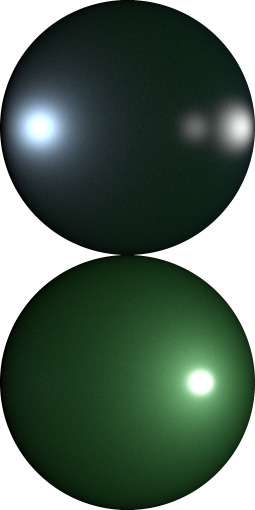
\includegraphics[width=0.315\columnwidth]{validations/lobe_bsdf/bsdf_sample_all.jpg} &
		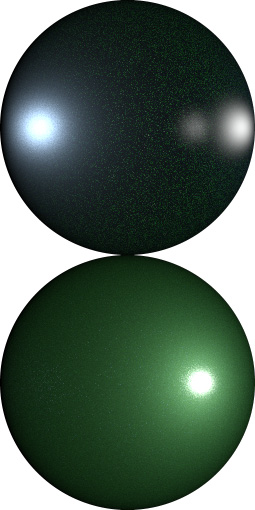
\includegraphics[width=0.315\columnwidth]{validations/lobe_bsdf/bsdf_eval_uni_all.jpg} &
		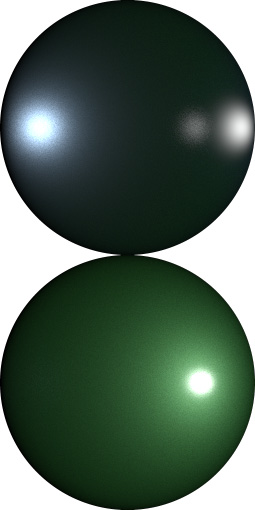
\includegraphics[width=0.315\columnwidth]{validations/lobe_bsdf/bsdf_eval_bi_all.jpg} \\
		Ground truth &
		Our unidir. &
		Our bidir. \\
	\end{tabular}
	\caption{\label{fig:hemispheres}
		\textbf{Outgoing lobes of a layered BSDF} (reflection and transmission) visualized as projected hemispheres. \textbf{Left:} ground truth computed by sampling and binning the light paths. \textbf{Middle:} Our unidirectional estimator. \textbf{Right:} Our bidirectional estimator (same time).
	}
\end{figure}

\begin{figure}[t]
	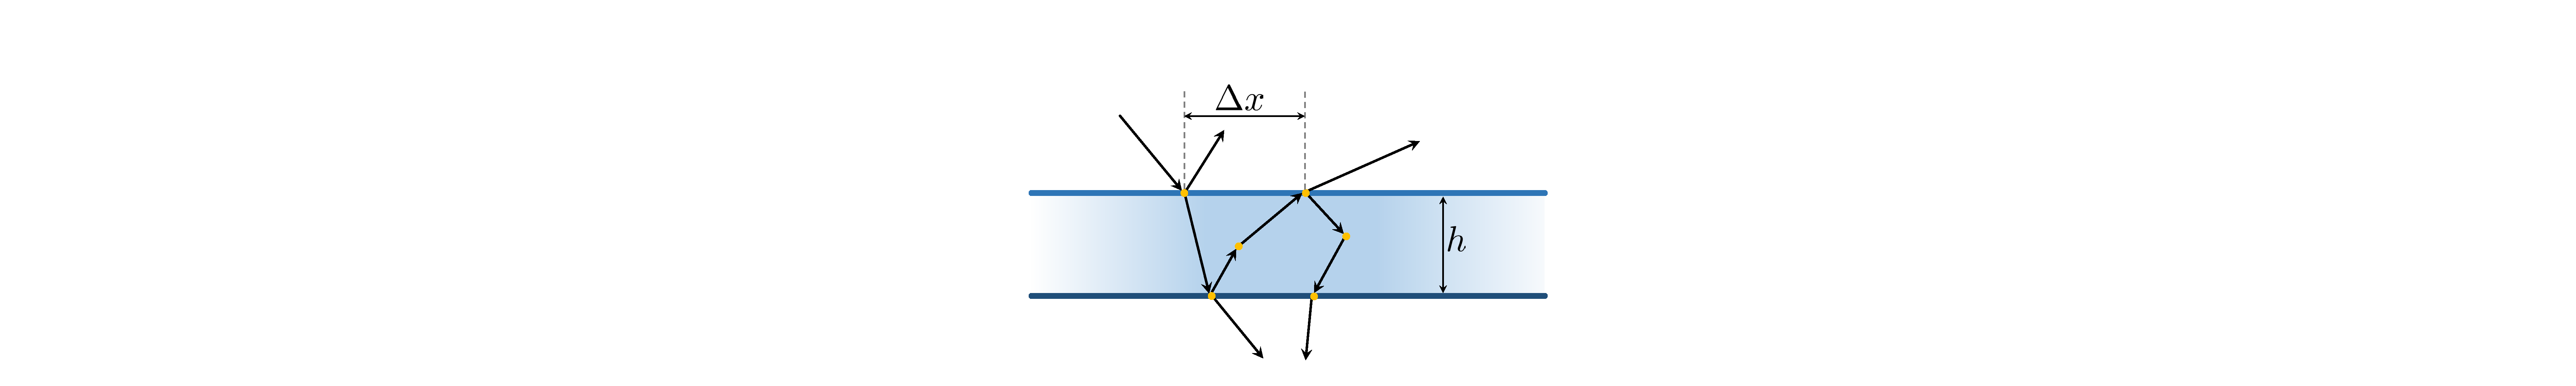
\includegraphics[width=0.6\columnwidth]{illustration/assumption.pdf}
	\caption{\label{fig:thin_layer}
		\textbf{Small displacement assumption:}
		when light hits a thin layer, it gets reflected and refracted by the interfaces and scattered and absorbed internally.
		Since the geometric thickness $h$ of the layer is small, we assume the displacements (e.g., $\Delta x$) of light's entrance and departure locations can be neglected.
	}
\end{figure}

In this section, we explicitly state the assumptions of our method, provide background on the standard path formulation of light transport, and provide a quick overview of the rest of the paper.

\subsection{Assumptions}

Although light generally enters and leaves the layer from different locations, we note that when the layers are thin and the lighting is comparably distant, the entrance and departure locations will be close enough to each other. We assume it is acceptable to ignore this displacement, allowing us to describe the light transport in the layers using BSDFs, rather than BSSRDFs (Figure~\ref{fig:thin_layer}).

Furthermore, we assume that the spatial variation of layer properties is slow enough that a BSDF evaluation at a single surface point can locally approximate them as spatially uniform. This is related to the above in assuming that the horizontal spreading of light is small enough to be negligible.

In fact, these are the \emph{only} approximating assumptions of our approach, which otherwise offers unbiased accuracy and full flexibility in setting the layer properties and varying them spatially.

\subsection{Review of Veach's path integral formulation}
\label{subsec:path_int}

In the Veach formulation of light transport~\shortcite{VeachThesis}, light paths are defined as sequences of vertices connected by segments.
The value of a light transport integral (for example, but not necessarily limited to, a pixel value) is written as
%
\begin{equation}
I = \int_\Omega f(\bar x) \intd \mu(\bar x),
\end{equation}
%
where $\bar x = (\bx_0, \dots, \bx_k)$ is a path with $k$ segments and $k + 1$ vertices on the surfaces or within the participating media of a scene.
$\Omega$ is the space of all paths and is defined as the union of $\Omega_k$ for $k \geq 0$, where $\Omega_k$ indicates the set of paths of length $k$.
Furthermore, $f(\bar x)$ is the path contribution to the integral, and $\mu(\bar x)$ is a special measure on the path space, defined as the product of area measures on the vertices $\bx_i$. The contribution $f(\bar x)$ is a product of vertex terms (normally BSDFs and phase functions) and geometry terms corresponding to path segments. The geometry terms contain the squared distance between the two vertices in the denominator; this is a significant source of variance when trying to connect independently sampled vertices on thin layer configurations.


\subsection{Paper overview}

In Section \ref{sec:path-formulation}, we describe our path formulation of layered light transport. Our path integral differs from Veach's formulation in that it is \emph{position-free}. The key idea is that on an infinite flat slab, the horizontal positions of vertices do not matter: it is only the vertical position (depth) of a vertex, and the \emph{directions} between vertices, that are relevant to a light transport integral. The vertices are defined by their depth in the layer, as opposed to a full 3D position, and the segments have variable unit directions.

It is important to note that our position-free formulation is not just a simplified specialization of the standard formulation to the flat slab setting, but in fact a new approach that achieves much superior variance to the standard formulation. The key benefit of this new formulation is that it does not contain the inverse square distance falloff terms that are required between any two vertices with full positional information. The leads to high variance, even in advanced estimators such as bidirectional and Metropolis transport, which in fact perform even worse in this setting than unidirectional; see Figure \ref{fig:validation1} for examples.

In contrast, our approach leads to an efficient estimator based on unidirectional sampling with next event estimation, and an even more efficient bidirectional estimator. The unidirectional performs similarly (though usually not better) in simpler cases, but in challenging cases with sharp and/or anisotropic BSDFs and phase functions, the bidirectional version is clearly more efficient (Figure~\ref{fig:validation1}, bottom). Figure \ref{fig:hemispheres} demonstrates the performance of the estimators through BSDF lobe visualization, also showing a close match to ground truth. In Section \ref{sec:ours}, we describe these two estimators in detail, and also focus on the two additional operations critical for integrating a BSDF into a practical renderer: importance sampling and pdf evaluation.

Finally, we present results in Section \ref{sec:results}, and summarize in Section \ref{sec:conclusion}.

% \subsection{Applying a Monte Carlo estimator}
% \label{sec:applymc}

% To evaluate the BSDF value $f_l(\omegain, \omegaout)$ for given query directions $\omegain$ and $\omegaout$, we need to evaluate the path integral of Eq.~\eqref{eq:pathintegral} by sampling paths $\bar x$ from some distribution, and weighting the paths by their contribution, divided by their probability densities in the measure $\mu(\bar x)$, i.e. the product of solid angle measures at the internal directions of the path.

% Consider the specific example of $\Omega_3(\omegain, \omegaout)$, i.e. the subspace of paths with three vertices, corresponding to a transmit-reflect-transmit (TRT) configuration.
% For paths in this subspace, only the directions $\bd_1$ and $\bd_2$ are ``free parameters'' participating in the integration, and the measure is simply the product of solid angle measures at $\bd_1$ and $\bd_2$.
% This suggests a simple and effective approach for choosing $\bd_1$ and $\bd_2$ (and thus $\bar x$): to importance-sample the top interface BSDF $f_\uparrow$ twice, by using $\omegain$ and $\omegaout$ as the incoming directions, respectively (Figure~\ref{fig:mis_local}-a).
% Alternatively, one can sample $\bd_1$ and $\bd_2$ by first drawing $\bd_1$ using $f_\uparrow$ (given $\omegain$) and then $\bd_2$ (given $\bd_1$) using $f_\downarrow$ (Figure~\ref{fig:mis_local}-b).
% This method is more efficient when the bottom interface is close to specular.
% Both strategies can be combined using MIS to provide a robust sampling scheme for light transport paths $\bar{x} \in \Omega_3(\omegain, \omegaout)$.

% In standard rendering systems, a BSDF sampling procedure commonly returns a ``weight'', defined as the BSDF value in the sampled direction $\bom$, times the cosine term, divided by the probability density (pdf) of picking the direction in the solid angle measure.
% %\szrem{Need a figure to make this part clearer.}
% This makes it particularly convenient to compute the path contribution divided by the pdf: simply multiply the two weights returned by importance-sampling $\bd_1$ and $\bd_2$, additionally multiplied by the BSDF at the bottom interface, $f_s(x_2, \bd_1, -\bd_2)$.

% Furthermore, it is clear that there is nothing specific about the TRT mode here, and a minor modification of this approach works for camera and light subpaths of any length. In our concrete implementation, the light subpath has up to one vertex, while the camera subpath can have any length.

%
\section{Position-Free Path Formulation: Definition and Derivation}
\label{sec:path-formulation}

In this section, we theoretically define the value of a layered BSDF due to a given layer stacking, for given query directions $\omegain$ and $\omegaout$, as a path integral. Given such a definition, any Monte Carlo method can be used to evaluate the BSDF by randomly sampling paths, evaluating their contributions and dividing by the corresponding probability density values.

\subsection{Notation}

We will use the notation $\cos \bom$ to denote the $z$-component of the unit vector $\bom$. We will also use $\ind(x)$ to denote an indicator function, returning 1 if the boolean condition $x$ is true and 0 if false. A bold font is used to denote unit vectors (directions) on $\Sph$. Please refer to Table \ref{tab:notation} for the notation used in this section.

\begin{figure}
	\centering
	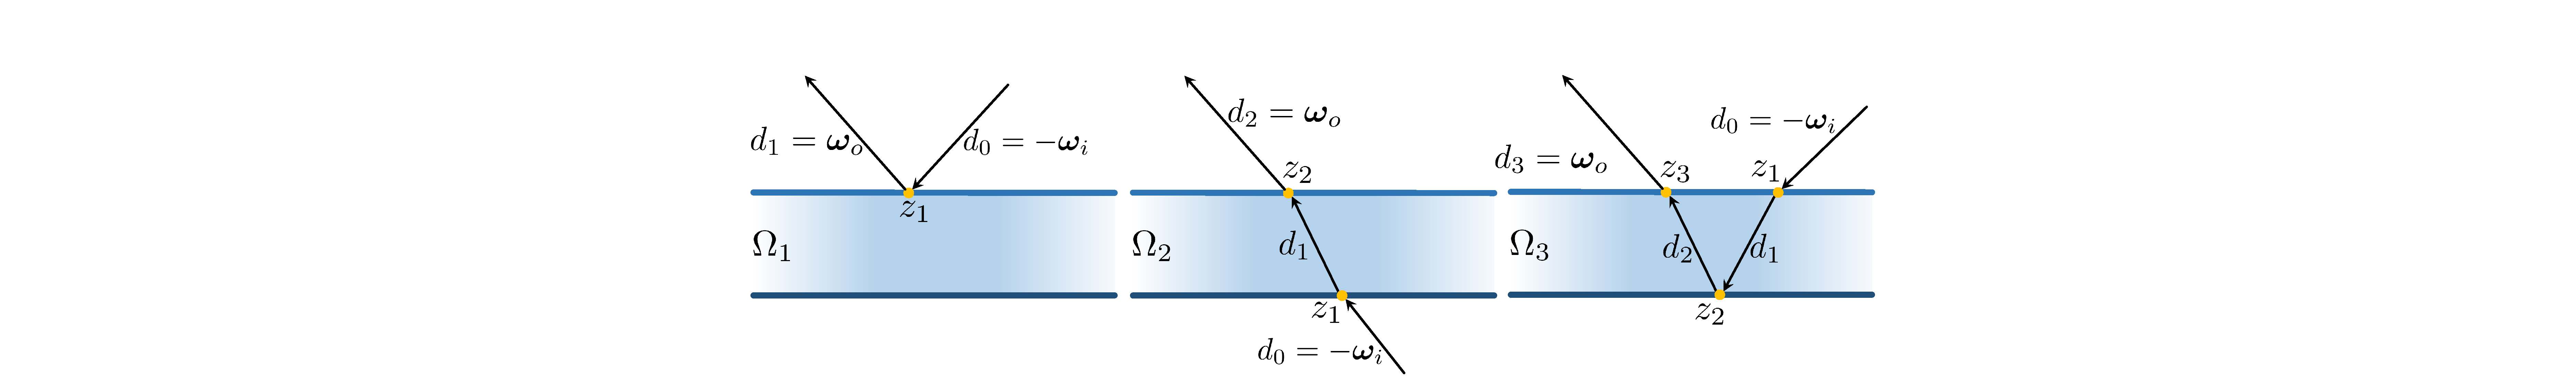
\includegraphics[width=\columnwidth]{illustration/omega.pdf}
	\caption{\label{fig:singlelayer}
		\textbf{Example paths} of lengths 1, 2 and 3.
		In our formulation, the exact positions of the vertices do not matter: the $z_i$ only carry information about which interface the vertex occurs on.
		The first and last in the sequence of directions $\bd_i$ map to the incoming and outgoing directions of the underlying BSDF query.
	}
\end{figure}


\subsection{Position-free path integral}

To develop the theory, we will first assume a single infinite flat slab with a BSDF $f_\uparrow$ on the top interface and a BSDF $f_\downarrow$ on the bottom interface, combined with a homogeneous scattering volume inside the slab to produce a resulting layered BSDF. The volumetric medium is defined by a phase function $f_p$, scattering coefficient $\sigma_s$ and extinction coefficient $\sigma_t$; we will use the notation $\hat f_p = \sigma_s f_p$.

For simplicity, we will drop the depth dependence of the volume parameters (though they could vary) and we will assume constant scattering / extinction coefficients, though they can vary with direction for fully anisotropic phase functions, which we also support. We will further assume that the slab has unit thickness; the formulation can be easily adjusted for any thickness.

A {\bf vertex} $z_i \in [0, 1]$ is a single real number indicating the depth within the layer. A value of 0 or 1 indicates a surface reflection or refraction event on the bottom or top interface, respectively. Fractional values indicate volume scattering events at the specified depth. Note again that the horizontal positions of vertices on the infinite flat interfaces are not needed.

A {\bf direction} $\bd_i$ is a unit vector on $\Sph$ denoting the light flow between vertices. In our convention (inherited from Veach), 
the vectors point in the direction of light flow (i.e. from light source to camera), and the vertex/direction indexing follows this as well.

A {\bf light path} $\bar x$ is a sequence of directions and vertices: $\bar x = (\bd_0,\ z_1,\ \bd_1,\ \dots,\ z_k,\ \bd_k)$.
 The first and last directions are aligned with the input and output directions of the layered BSDF query, i.e. $\bd_0 = -\omegain$ and $\bd_k = \omegaout$. In contrast to Veach's formulation, the path interleaves directions with vertices, and the two ends of the path are defined by directions (not vertices). See Figure \ref{fig:singlelayer} for some example paths.

The {\bf path contribution} $f(\bar x)$ of a light path is the product of vertex terms $v_i$ (on each vertex) and segment terms $s_i$ (on all internal segments):
%
\begin{equation}
	f(\bar x) = v_1 s_1 v_2 s_2 \dots s_{k-1} v_k.
\end{equation}
%
The vertex term consists of the BSDF or phase function value:
%
%\begin{eqnarray}
%v_i & = & f_\uparrow(\bd_{i-1}, -\bd_i) \mbox{  if  } z_i = 1, \\
%    & = & f_\downarrow(\bd_{i-1}, -\bd_i) \mbox{  if } z_i = 0, \\
%    & = & \hat f_p(\bd_{i-1}, -\bd_i) \mbox{  if  } 0 < z_i < 1.
%\end{eqnarray}
%
\begin{equation}
\label{eqn:vtx_contrib}
v_i = v(z_i, -\bd_{i - 1}, \bd_i)
= \begin{cases}
	f_\uparrow(-\bd_{i-1}, \bd_i)   & \mbox{  if  } \sz{z_i = 0},\\
	f_\downarrow(-\bd_{i-1}, \bd_i) & \mbox{  if  } z_i = 1,\\
  	\hat{f}_p(-\bd_{i-1}, \bd_i)    & \mbox{  if  } 0 < z_i < 1.
\end{cases}
\end{equation}
%
Define \sz{the} transfer term $\tau(z_1, z_2, \bom)$ as follows:
\begin{equation}
\tau(z, z', \bom) := \exp \left( \frac{-\sigma_t |z' - z|}{|\cos \bom|} \right) \cdot \ind \left( \frac{z' - z}{\cos \bom} > 0 \right).
\end{equation}
%
The purpose of the exponential term is to compute the transmittance when going from depth $z$ to $z'$ following direction $\bom$.
The indicator term checks the validity of the configuration (i.e. if the direction points up, then $z'$ should be greater than $z$, and vice versa). The segment term for internal segments can now be defined as:
%
\begin{equation}
\label{eqn:seg_contrib}
s_i = s(z_i, z_{i + 1}, \bd_i) := \tau(z_i, z_{i+1}, \bd_i) \cdot |\cos \bd_i|^{\alpha_i},
\end{equation}
where
\begin{equation}
\label{eqn:seg_contrib_cosine}
\alpha_i = \ind(z_i \in \{0,1\}) + \ind(z_{i + 1} \in \{0,1\}) - 1.
\end{equation}
%
This definition encapsulates the subtle behavior of cosine terms along the path segments.
\sz{For a detailed derivation, please refer to Appendix~\ref{sec:derivation}.}
\begin{comment}
A segment between two layer interface vertices will have a single cosine term, a segment between two volume scattering vertices will have a cosine term in the denominator, and a mixed interface/volume segment will have no cosine term. Note the symmetry of this definition with respect to light/camera reversal. The reason for this behavior can be found in the derivation below.
\end{comment}

The {\bf path space} $\Omega(\omegain, \omegaout)$ is the set of all paths of one or more vertices, such that the first direction of the path is equal to $-\omegain$ and the last to $\omegaout$. It can be seen as the union of the spaces of such paths of all lengths $k \geq 1$, that is, $\Omega = \cup_{k \geq 1} \Omega_k$.

The {\bf path space measure} $\mu(\bar x)$ is a product of solid angle measures $\sigma$ on the internal directions of the path, times the product of line measures $\lambda$ on volumetric scattering vertices.
That is, for a $k$-vertex path,
\begin{equation}
\mu(\bar x) = \prod_{i=1}^{k-1} \sigma(\bd_i) \cdot \prod_{i \in V(\bar x)} \lambda(z_i).
\end{equation}
Here $V(\bar x)$ is the set of indices of volumetric vertices on $\bar x$, and $\lambda$ is the line measure (i.e. standard Lebesgue measure on the real numbers).

Finally, we can define the {\bf layered BSDF value} $f_l(\omegain, \omegaout)$ as an integral over the set of paths $\Omega(\omegain, \omegaout)$:
%
\begin{equation}
\label{eq:pathintegral}
	f_l(\omegain, \omegaout) = \int_{\Omega(\omegain, \omegaout)} f(\bar x) \intd \mu(\bar x).
\end{equation}
%
As usual, any Monte Carlo method can be used to compute this integral. As long as the probability density $p(\bar x)$ with respect to measure $\mu(\bar x)$ of generated sample paths is known, we simply average a number of samples of the form $f(\bar x) / p(\bar x)$.

\begin{table}
	\caption{Notation used in the path formulation (\S\ref{sec:path-formulation}).}
	\label{tab:notation}
	\begin{tabular}{ll}
		$\omegain$ & light direction \\
		$\omegaout$ & camera direction \\
		$\cos \bom$ & $z$-component of the unit vector $\bom$ \\
		$\ind(x)$ & binary indicator function \\
		\hline
		
		$f_l(\omegain, \omegaout)$ & layered BSDF (our goal) \\
		$f_s(z, \omegain, \omegaout)$ & interface BSDF at depth $z$ \\
		$f_\uparrow, f_\downarrow$ & BSDFs $f_s$ at top and bottom interface \\
		$f_p(\omegain, \omegaout)$ & phase function (normalized as a pdf) \\
		$\sigma_s, \sigma_t$ & scattering and aborption coefficient \\
		$\hat f_p$ & reduced phase function, $\hat f_p = \sigma_s f_p$ \\
		\hline
		
		$z_i$ & depth of $i$-th path vertex \\
		$\bd_i$ & direction of $i$-th path segment \\
		$\bar x$ & light path $(\bd_0,\ z_1,\ \bd_1,\ \dots,\ z_k,\ \bd_k)$ \\
		$v_i$ & $i$-th vertex contribution \\
		$s_i$ & $i$-th segment contribution \\
		$\tau(z, z', \bom)$ & transfer through segment \\
		$\alpha_i$ & $i$-th segment cosine term exponent \\
		$\mu(\bar x)$ & path space measure \\
		$\sigma(\bom)$ & solid angle measure on unit directions \\
		$\lambda(z)$ & line (Lebesgue) measure on real numbers \\
		$p(\bar x)$ & pdf of path $\bar x$ in measure $\mu(\bar x)$ \\
		\hline
		
		$L_v(z, \omegaout)$ & volume radiance \\
		$L_s(z, \omegaout)$ & outgoing surface radiance \\
		$L^i_s(z, \omegain)$ & incoming surface radiance \\
		$S(z, \bom)$ & source term in radiative transfer eq. \\
	\end{tabular}
\end{table}



\subsection{Derivation}

Here we sketch the derivation of the path formulation.
%An expanded derivation can be found in the supplementary document. \todo{do we need that?}
Like in Veach's version (and its volumetric extension), the derivation proceeds by recursively expanding the surface and volume rendering equation (the latter also commonly known as the radiative transfer equation). Denote the surface radiance by $L_s(z, \bom)$ (for $z \in \{0, 1\}$) and the volume radiance $L_v(z, \bom)$ (for $z \in [0,1]$).

The volume radiance will satisfy the standard radiative transfer equation, specialized to our position-free setting:
%
\begin{multline}
\label{eq:IRTE}
L_v(z, \bom) = S(z, \bom) \ + \\
\int_0^1 \frac{\tau(z', z, \bom)}{|\cos\bom|} \, \, \int_{\Sph} \hat f_p(\bom', \bom) \, L_v(z', \bom') \,\intd \bom' \intd z',
\end{multline}
%
where the source term $S(z, \bom)$ gives illumination from the boundary of the slab:
%
\begin{equation}
S(z, \bom) = \tau(0, z, \bom) L_s(0, \bom) \ + \ \tau(1, z, \bom) L_s(1, \bom).
\end{equation}
%
Notice that, although the source term has two components, only one of them will be non-zero for any given query.
This formulation is valid even with no scattering within the layer, in which case $\hat f_p = 0$ and the second term of Eq.~\eqref{eq:IRTE} vanishes.
\sz{Further, the $1/|\cos\bom|$ factor is due to a change of variable (from free-flight distance to depth). For more details, please refer to Appendix~\ref{sec:derivation}.}

The surface radiance $L_s(z, \bom)$ satisfies the standard rendering equation:
%
\begin{equation}
\label{eq:RE}
L_s(z, \bom) = \int_{\Sph} f_s(z, \bom, \bom') \ |\cos \bom'| \ L_s^i(z, \bom') \intd \sigma(\bom'),
\end{equation}
where $L_s^i(z, \bom')$ is the incoming surface radiance. In case the incoming radiance query points back into the layer, we have
\begin{equation}
\label{eq:incoming}
L_s^i(z, \bom) = L_v(z, -\bom).
\end{equation}

The BSDF value is defined as the radiance leaving the surface in direction $\omegaout$, under unit irradiance from a directional light in direction $\omegain$. This is equivalent to evaluating $L_s(1, \omegaout)$ under the boundary condition
%
\begin{equation}
	\label{eq:bound}
	L_s^i(z, \bom) = \frac{\delta(\bom - \omegain)}{|\cos \omegain|}.
\end{equation}
%
One can easily check that the irradiance under this illumination is unit. Thus the incoming surface radiance $L^i_s$ is given by Eq.~\eqref{eq:bound} when $\bom$ points out of the layer and Eq.~\eqref{eq:incoming} when it points back into the layer.

The path formulation can now be obtained by recursively expanding the desired value $L_s(1, \omegaout)$ using the above equations for $L_s$ and $L_v$, terminating the paths using the boundary condition. Note that:
\begin{itemize}
	\item Each recursive expansion of Eqs.~\eqref{eq:IRTE} or \eqref{eq:RE} will contribute an $\hat f_p$ or $f_s$ term, respectively, to the path vertex.
	\item Each volumetric segment will introduce a $\tau(z, z', \bom)$ term, whether the first or second term in Eq.~\eqref{eq:IRTE} is taken.
	\item{Expanding the rendering equation contributes a cosine term to the \emph{next} segment, while expanding the radiative transfer equation contributes a 1/cosine term to the \emph{previous} segment. A combination of these contributions explains the $\alpha_i$ term above.}
	\item The last surface cosine is canceled out when using the boundary condition, due to the denominator cosine in Eq.~\eqref{eq:bound}.
\end{itemize}



\subsection{Normal mapping}

An important feature of our method is the mapping of normals of the layer interfaces, introducing mismatches between geometric (flat) normals and shading (mapped) normals. The definition of the segment term (Eq.~\eqref{eqn:seg_contrib}) changes with the presence of shading normals. Precisely, it becomes
\begin{equation}
s_i = \tau(z_i, z_{i+1}, \bd_i) \ \frac{|\langle \bn(z_i), \bd_i \rangle| \ |\langle \bn(z_{i + 1}), \bd_i \rangle|}{|\cos \bd_i|},
\end{equation}
where $\bn(z)$ denotes the local shading normal at $z$ (for $z \in \{0, 1\}$). This term is no longer symmetric, which implies that BSDFs with mapped normals will in general not be reciprocal. When sampling paths from the light, it is important to handle such BSDF using the correction term introduced by Veach \shortcite{VeachThesis} (Eq.~5.19).


\subsection{Note about reciprocity}

Our layered BSDF will be reciprocal whenever the path contribution $f(\bar x)$ is symmetric with respect to the reversal of the path. Assuming normal mapping is not used, the segment term $s_i$ will be symmetric, so the reciprocity boils down to the symmetry of the vertex terms $v_i$. This will certainly hold if all phase functions and BSDFs are reciprocal.

Note, however, that crossing an interface between regions of different index of refraction (whether smooth or rough) is not reciprocal in the usual sense. Instead, a physical refractive BSDF should obey a modified reciprocity relation $f_s(\omegain, \omegaout) = \eta_o^2 / \eta_i^2 \cdot f_s(\omegaout, \omegain)$ \cite{Walter:2007:MMR}, where $\eta_i$ and $\eta_o$ are the refractive indices of the corresponding media. In the common case where the layered BSDF's incoming and outgoing directions are both assumed to be in air, the final layered BSDF will still be reciprocal, because there will be an equal number of $\eta^2$ and $1/\eta^2$ terms along the path for each medium with index $\eta$.


\subsection{Multiple slabs}
\label{subsec:multi_layer}

Finally, we support extending the framework to multiple slabs. This is relatively straightforward theoretically, and simply requires explicitly keeping track of the interface or volume that a vertex/segment belongs to. We also need to modify the transfer term $\tau(z,z'\bom)$ to return zero in cases when the segment crosses an internal interface.

Another option to obtain a multi-layer BSDF is by recursively nesting the BSDFs. To construct the layered BSDF due to a layer stacking of $n$ slabs, we define the layered BSDF due to the stacking of the bottom $n-1$ slabs, and use this BSDF as the bottom interface's BSDF in adding the top layer according to the above theory. We have found that this approach works in practice, but its performance is worse than the explicit implementation above.
%\sz{For example, for Figure~\ref{fig:validation1} (bottom), using the explicit method is about $2\times$ as fast as using the nested one.}



%
\section{Our Estimators}
\label{sec:ours}
%
We now describe our specific layered BSDF method,
%This can be seen as a specific Monte Carlo estimator based on the formulation depicted in \S\ref{sec:path-formulation}.
%Standard rendering frameworks require at least two key operations to fully define a BSDF model: 
by presenting our Monte-Carlo solutions to enable the three key operations needed to fully define a BSDF model:
sampling (\S\ref{subsec:ours_sample}), evaluation (\S\ref{subsec:ours_eval}) and pdf computation (\S\ref{subsec:ours_pdf}).
Sampling produces the outgoing direction $\omegaout$ given the incoming one $\omegain$ (or the reverse), while evaluation answers the BSDF query for given $\omegain$ and $\omegaout$. Note that the values returned from sampling, evaluation and pdf procedures are themselves stochastic, and are equal to the true BSDF value, pdf value or sampling weight only in expectation. Stochastic evaluation was also used in some recent BSDF models \cite{Heitz:2016:MMB}. 

Multiple importance sampling (MIS) is commonly used to combine multiple techniques to produce a given path, and key to obtaining low-noise results under complex lighting conditions. This technique typically uses the sampling pdfs of the techniques being combined to derive the weights, which requires the pdf values of the layered BSDFs. We introduce two solutions: an unbiased solution for estimating the exact pdf values in expectation, as well as a fast and approximate version which we demonstrate is sufficient for MIS (\S\ref{subsec:ours_pdf}). \sz{In a supplementary document, we show that the estimators are still unbiased in the presence of approximate pdfs for MIS weighting and stochastic evaluation of both weights and function values.}

\begin{figure*}[t]
	\centering
	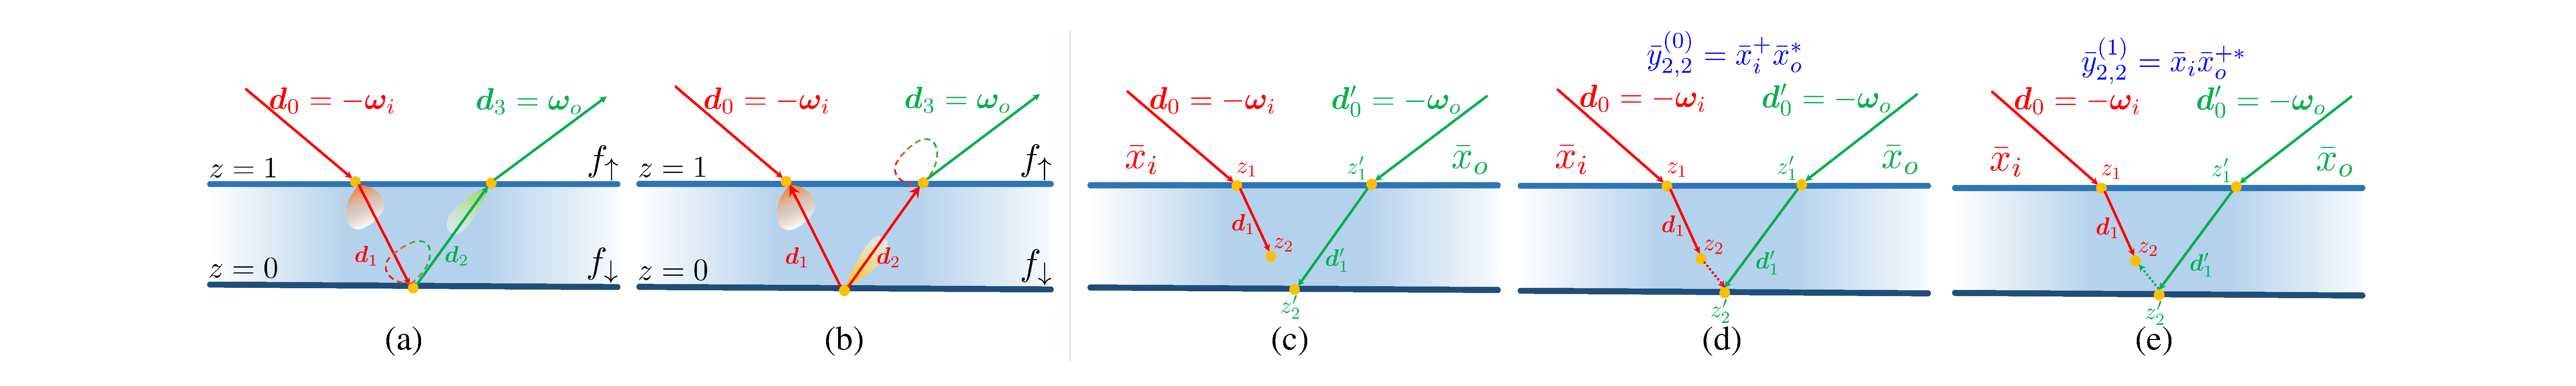
\includegraphics[width=\textwidth]{img/illustration/unidir-bidir.pdf}
	\caption{
		\label{fig:estimators}
		\textbf{Our Monte Carlo estimators} for BSDF values.
		\textbf{(ab)} Unidirectional estimator uses two path sampling strategies for ``shading'' a vertex on the bottom layer:
		(a)~sampling the BSDF $f_\uparrow$ of the top interface and connecting at the bottom (next event estimation); or (b)~sampling $\bd_2$ using $f_\downarrow$ and connecting at the top (path continuation). These strategies are combined using local MIS. \textbf{(cde)} Bidirectional estimator: (c) Two subpaths with initial directions $\omegain$ and $\omegaout$. (de) Two full light paths constructed by sampling an additional direction from each sub-path.
	}
\end{figure*}



\subsection{BSDF sampling}
\label{subsec:ours_sample}
%
Sampling a BSDF is the problem of drawing the outgoing direction $\omegaout$ given the incoming one $\omegain$ (or the reverse), with a pdf proportional, exactly or approximately, to the value $f_l(\omegain, \omegaout)$ (times the cosine term, if possible).
This is straightforward: we draw $\omegaout$ simply by following the stochastic process given by light interacting with the layered configuration.
That is, we utilize a pure forward path tracing process that starts with a ray with direction $-\omegain$ and explicitly simulates interactions between the ray and the layer's interfaces and internal media by sampling the corresponding BSDFs and phase functions, accumulating a throughput value along the way.
When the ray eventually leaves the layer, its direction gives $\omegaout$ and the throughput of the full light transport path gives the stochastic sample weight. Formally, this weight is an estimate of the BSDF value, times the exitant cosine direction, divided by the sampling pdf in solid angle measure.

Although this simulation is analogous to standard Monte Carlo path tracing, it is usually much more efficient than tracing paths in the global scene thanks to the simplicity of the flat slab configuration (under which ray tracing becomes simple numerical computation, not requiring any acceleration structures).

\subsection{BSDF evaluation}
\label{subsec:ours_eval}
%
To evaluate our BSDF $f_l$ at given incoming and outgoing directions $\omegain$ and $\omegaout$, we introduce two Monte Carlo based methods to evaluate the path integral from Eq.~\eqref{eq:pathintegral}.
The first one (\S\ref{sssec:ours_unidir}) is analogous to a unidirectional path tracer with next-event estimation (NEE), while the second (\S\ref{sssec:ours_bidir}) uses a bidirectional scheme.

\subsubsection{Unidirectional simulation}
\label{sssec:ours_unidir}
%
In standard path tracing, a shading point would be directly connected to a light source in a process often called \emph{direct illumination} or \emph{next event estimation} (NEE), which is crucial for low-variance rendering. In an analogy to this technique, consider a shading point inside a single layer slab (whether on the bottom interface or a scattering point within the medium). We would like to create a path ending with $\omegain$, intuitively connecting it to an external directional light source with direction $\omegain$. However, direct connection between the shading point and the desired external direction is usually invalid due to the layer's top refractive interface.

To address this problem, we introduce our NEE scheme that directly connects scattering events across potentially rough refractive interfaces.
Assume without loss of generality that our path tracing starts with direction $\omegaout$.
At each scattering event, we need to find a direction $\omegain'$ so that $\omegain \to \omegain'$ follows the BSDF at the interface.
To this end, we draw $\omegain'$ by sampling the interface BSDF backwards, given $\omegain$.
Finally, we simply multiply the accumulated throughput by the weight returned from the sampling routine, and the BSDF (or phase function) value at the scattering event.

Furthermore, this NEE connection can be combined with a path continuation (by sampling the phase function or interface BSDF), using MIS for the weighting. This is analogous to the MIS direct illumination used in many practical path tracers, with the difference that the path can cross a refractive boundary. Note the distinction between this \emph{local} MIS, and the \emph{global} MIS used by the scene-level transport algorithm (a standard path tracer in our results). An illustration of these two techniques, applied to a transmit-reflect-transmit (TRT) configuration, can be found in Figure \ref{fig:estimators}-ab.

Previous work on next-event estimation in scattering volumes through refractive interfaces \cite{Walter2009,Koerner2016} is related to our scheme, but focuses on arbitrary geometries, which is not necessary in the flat layer setting.

Extending this NEE scheme to cross multiple layer interfaces is somewhat tedious to implement, as care must be taken not to double-count light paths. We instead use the recursive nesting approach to multiple layers (\S\ref{subsec:multi_layer}) when using the unidirectional estimator, which handles these issues automatically.

%Note that this ``backward'' sampling is conceptually similar to bidirectional path tracing (i.e. sampling an additional path segment from the light). However, the fact that only directions between vertices matter (and not their horizontal positions) works significantly in our favor, because we can never ``miss'' the shading point by backward sampling, nor do we have to solve for the position of a connecting vertex like Walter et al.'s approach for refraction through triangle mesh boundaries \shortcite{Walter2009}. Note, in practice, one should be careful to use the correct ``transport'' mode of the BSDF when sampling it from the camera and/or from the light; this makes a difference for refractive transmission due to the non-reciprocity discussed in \S\ref{sec:background}.

% Unlike traditional BSDFs that are evaluated deterministically, the evaluations of our BSDFs are stochastic.
% Fortunately, the additional variance introduced by our stochastic evaluation is usually minor thanks to our effective NEE technique.
% Compared to explicitly simulating the layered geometry, our technique offers much better convergence. (see Figure~\todo{XXX}).




% \begin{figure}[t]
% 	\centering
% 	\includegraphics[width=\columnwidth]{img/illustration/bidir.pdf}
% 	\caption{\label{fig:bidir0}
% 		\textbf{Our bidirectional estimator.}
% 		(a) Two subpaths with initial directions $\omegain$ and $\omegaout$;
% 		(bc) Two full light paths constructed by sampling an additional direction from each sub-path.
% 	}
% \end{figure}

\subsubsection{Bidirectional simulation}
\label{sssec:ours_bidir}
%
Although our unidirectional solution works well in many cases, we introduce a new bidirectional approach that performs even better.
Our approach is conceptually similar to bidirectional path tracing (BDPT) but is technically different in several ways due to our position-free path formulation.

Given the incoming and outgoing directions $\omegain$ and $\omegaout$, consider two light transport paths, generated from the light and camera, respectively.
%
\begin{equation}
\begin{aligned}
% \bar{x}_i &= (\bd_0, z_1, \bd_1, \ldots, z_{n_i}, \bd_{n_i}),\\
% \bar{x}_o &= (\bd'_0, z'_1, \bd'_1, \ldots, z'_{n_o}, \bd'_{n_o}),
\bar{x}_i &= (\bd_0, z_1, \bd_1, \ldots, z_s) \\
\bar{x}_o &= (\bd'_0, z'_1, \bd'_1, \ldots, z_t'),
\end{aligned}
\end{equation}
%
where $\bd_0 = -\omegain$ and $\bd'_0 = -\omegaout$ (Figure~\ref{fig:estimators}-c).
%Then, for each $1 \leq s \leq n_i$ and $1 \leq t \leq n_o$,
Now we can construct a full light path $\bar{y}_{s, t}$ connecting the $s$-th vertex in $\bar{x}_i$ and the $t$-th vertex in $\bar{x}_o$ (assuming the connection between $z_s$ and $z'_t$ does not cross any layer boundary):
%
\begin{equation}
\bar{y}_{s, t} = (\bd_0, \ldots, z_{s - 1}, \bd_{s - 1}, z_s, \tilde{\bd}, z'_t, -\bd'_{t - 1}, z'_{t - 1}, \ldots, -\bd'_0).
\end{equation}
%
Unlike traditional BDPT, where the connection term between two given subpaths endpoints is fixed, there exists infinitely many valid directions $\tilde{\bd}$ connecting $z_s$ and $z'_t$ in our case, which gives us freedom to importance-sample the direction. In practice, we choose $\tilde{\bd}$ in two ways by sampling additional directions $\bd_s$ and $\bd'_t$ by extending the two subpaths with an extra importance sampling step. We set $\tilde{\bd}$ to $\bd_s$ and $-\bd'_t$ respectively. This yields two light paths $\bar{y}^{(0)}_{s, t}$ and $\bar{y}^{(1)}_{s, t}$ (Figure~\ref{fig:estimators}-de), thus providing two samples of the path integral.
Denote the extended subpaths by
%
\begin{align}
\bar{x}_i^+ &:= (\bd_0, z_1, \bd_1, \ldots, z_s, \bd_s),\\
\bar{x}_o^+ &:= (\bd'_0, z'_1, \bd'_1, \ldots, z'_t, \bd'_t),
\end{align}
%
and let $\bar{x}^*$ denote the adjoint (reversed) version of a light path $\bar{x}$, e.g., $\bar{x}_o^{+*} = (-\bd'_t, z'_t, -\bd'_{t - 1}, \ldots, z'_1, -\bd'_0)$.

Let $v(z, \bom, \bom')$ and $s(z, z', \bom)$ be the vertex and segment contributions defined in eqs.~\eqref{eqn:vtx_contrib} and \eqref{eqn:seg_contrib}.
We can easily verify that
%
\begin{align}
f(\bar{y}_{s,t}^{(0)}) &= f(\bar{x}_i^+) \, f(\bar{x}_o^*) \, s(z_s, z'_t, \bd_s) \, v(z'_t, -\bd_s, -\bd'_{t - 1}),\\
f(\bar{y}_{s,t}^{(1)}) &= f(\bar{x}_i) \, f(\bar{x}_o^{+*}) \, v(z_s, -\bd_{s - 1}, -\bd'_t) \, s(z_s, z'_t, -\bd'_t).
\end{align}
%
It follows that the two Monte Carlo estimates will be:
%
\begin{align}
\label{eqn:bidir_estimate_i}
\frac{f(\bar{y}^{(0)}_{s, t})}{p(\bar{y}^{(0)}_{s, t})} &=
\frac{f(\bar{x}_i^+)}{p(\bar{x}_i^+)}
\frac{f(\bar{x}_o^*)}{p(\bar{x}_o)}
\, s(z_s, z'_t, \bd_s) \, v(z'_t, -\bd_s, -\bd'_{t - 1})\\
%
\label{eqn:bidir_estimate_j}
\frac{f(\bar{y}^{(1)}_{s, t})}{p(\bar{y}^{(1)}_{s, t})} &=
\frac{f(\bar{x}_i)}{p(\bar{x}_i)}
\frac{f(\bar{x}_o^{+*})}{p(\bar{x}_o^+)}
\, v(z_s, \bd_{s - 1}, \bd'_t) \, s(z_s, z'_t, -\bd'_t),
\end{align}
Note that in general $f(\bar x_o) \neq f(\bar x_o^*)$ and $f(\bar x_o^+) \neq f(\bar x_o^{+*})$ due to non-reciprocal operations such as shading normals; care must be taken to compute correct throughputs of light subpaths, as detailed in Chapter 5 of Veach \shortcite{VeachThesis}.

The above discussion assumed a single light and single camera subpath. In practice, we combine all prefixes of the sampled subpaths. In particular, we sample subpaths of length $n_i$ and $n_o$ from the light and camera respectively (the lengths are chosen through Russian roulette):
\begin{equation}
\begin{aligned}
\bar{x}_i &= (\bd_0, z_1, \bd_1, \ldots, z_{n_i}, \bd_{n_i}),\\
\bar{x}_o &= (\bd'_0, z'_1, \bd'_1, \ldots, z'_{n_o}, \bd'_{n_o}).
\end{aligned}
\end{equation}
For all $s$ and $t$ combinations, Eqs.~\eqref{eqn:bidir_estimate_i} and \eqref{eqn:bidir_estimate_j} provide $2 n_i n_o$ estimators of $f_l(\omegain, \omegaout)$.
Combining them using MIS gives us our bidirectional estimator for paths of length 2 or more vertices. We handle single vertex paths separately. The details of MIS weighting are discussed in the supplementary document.

% MIS pdf comparison figure
\begin{figure*}[t]
	\addtolength{\tabcolsep}{-4pt}
	\begin{tabular}{ccc}
		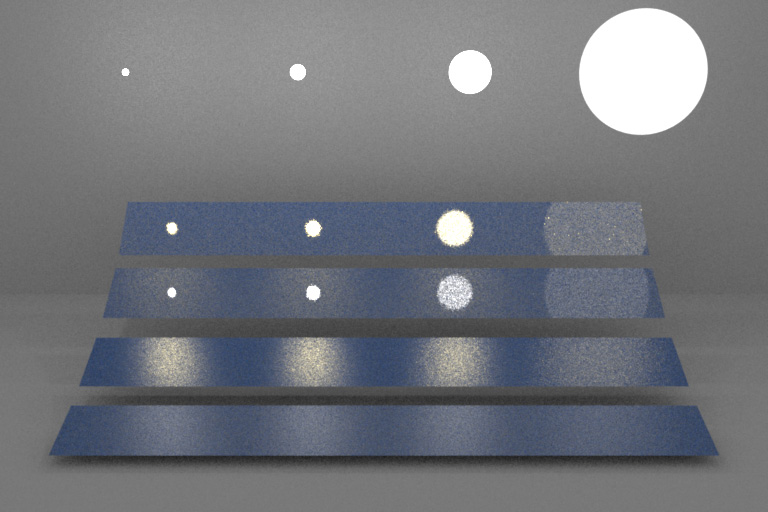
\includegraphics[width=0.32\textwidth]{validations/mis/mi_acr_64spp_14min.jpg} & 
		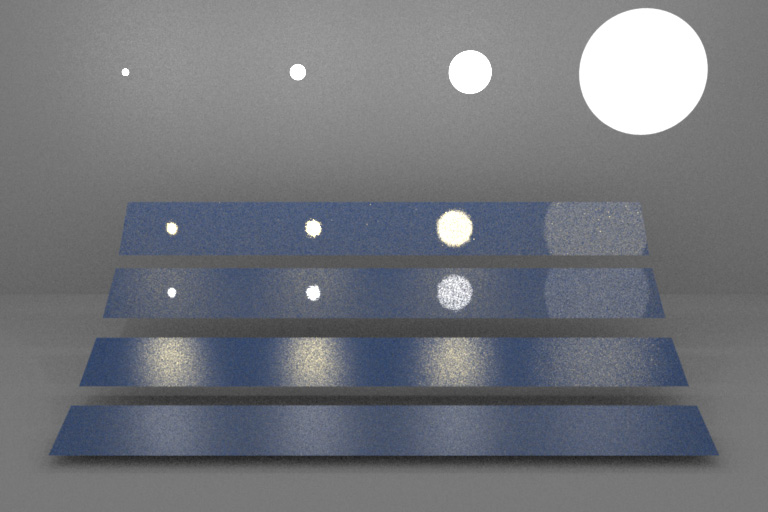
\includegraphics[width=0.32\textwidth]{validations/mis/mi_trt_64spp_4_1min.jpg} & 
		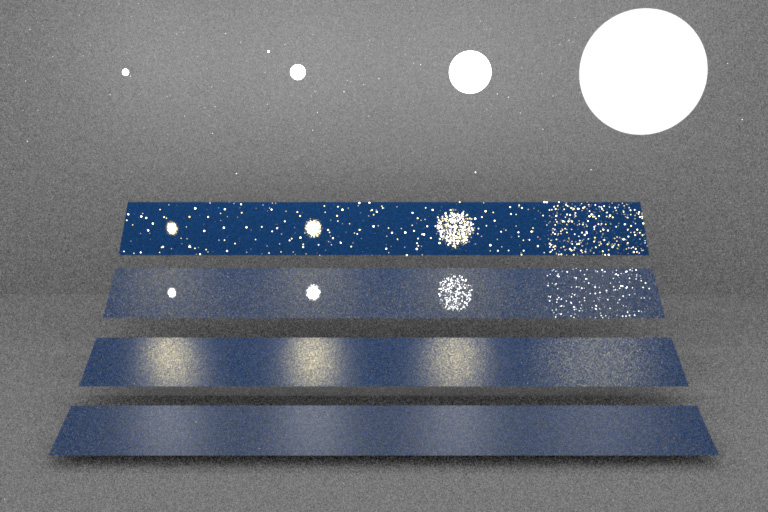
\includegraphics[width=0.32\textwidth]{validations/mis/mi_noMIS_80spp_4_2min.jpg} \\
		MIS + unbiased pdf (14 min) &
		MIS + approx. pdf (4 min) &
		no MIS (4 min) \\ 
	\end{tabular}
	\caption{
		\textbf{Multiple importance sampling} using our BSDFs.
		\sz{The slabs in this figure use a layered material with rough dielectric on the top, rough gold conductor on the bottom, and blueish homogeneous scattering medium in between.}
		\textbf{Left:} Using the unbiased pdf from \S\ref{sssec:ours_pdf_unbiased} for MIS in a traditional global path tracer. \textbf{Middle:} Using the approximate pdf from \S\ref{sssec:ours_pdf_approx} is faster and gives equivalent quality. \textbf{Right:} Using no MIS is clearly inferior.}
	\label{fig:pdf-eval}
\end{figure*}


\subsection{Pdf estimation}
\label{subsec:ours_pdf}

Another important operation for practical BSDF models is to evaluate the probability density for sampling provided incoming and outgoing directions.
That is, to evaluate $p(\omegaout \;|\; \omegain)$, the probability density of $\omegaout$ given $\omegain$ (assuming that the sampling process draws $\omegaout$ and fixes $\omegain$).
This operator \sz{is used for weight computation in} multiple importance sampling (using balance or power heuristics), a crucial technique for generating low-noise results using scene-level Monte Carlo rendering techniques. Note that this pdf is in the solid angle measure; it is a marginal pdf distinct from the path pdf $p(\bar x)$.

Although $p(\omegaout \;|\; \omegain)$ is usually easily available for traditional analytical BSDFs, no closed-form pdf exists in our case. Instead, the pdf evaluation has comparable form to the BSDF evaluation itself. It can be expressed using another position-free path integral:
%
\begin{equation}
\label{eqn:ours_pdf}
p(\omegaout \;|\; \omegain) = \int_{\Omega(\omegain, \omegaout)} \mathcal{P}(\bar{x}) \intd\mu(\bar{x}),
\end{equation}
%
where
%
\begin{equation}
\mathcal{P}(\bar{x}) := \left(\prod_{j = 1}^k p(\bd_j \;|\; z_j, \bd_{j - 1})\right) \left(\prod_{j = 1}^{k - 1} p(z_{j + 1} \;|\; z_j, \bd_{j - 1})\right),
\end{equation}
%
with $k$ denoting the number of vertices in $\bar{x}$. Note that $\bd_k = \omegaout$.

We introduce two nondeterministic methods, an unbiased~(\S\ref{sssec:ours_pdf_unbiased}) and a fast approximate approach~(\S\ref{sssec:ours_pdf_approx}), to estimate $p(\omegaout \;|\; \omegain)$.
These operations are not used in standard Monte Carlo light transport and are new, to our knowledge.
In practice, the approximate approach can be used when exact estimations are unnecessary (as is the case for a global path tracer with MIS, which we use for our results).
\sz{
	Note that the estimated $p(\omegaout \;|\; \omegain)$ is only ever used for MIS weight computation.
	We never use approximate path pdfs for Monte Carlo estimates, as this would introduce bias.
	Our BSDF value estimators directly return path throughput with accurate pdf factored in.
	% $f(\bar{x})/\mathcal{P}(\bar{x})$
}

\subsubsection{Unbiased pdf estimation}
\label{sssec:ours_pdf_unbiased}
%
Both our Monte Carlo estimators introduced in \S\ref{sssec:ours_unidir} and \S\ref{sssec:ours_bidir} can be adapted to estimate the path integral in Eq.~\eqref{eqn:ours_pdf} in an unbiased manner.
For instance, the estimators given by Eqs.~\eqref{eqn:bidir_estimate_i} and \eqref{eqn:bidir_estimate_j} simply require a replacement of $f$ by $\mathcal P$, and become:
%
\begin{align}
	\label{eqn:bidir_pdf_i}
	\frac{\mathcal{P}(\bar{y}^{(0)}_{s, t})}{p(\bar{y}^{(0)}_{s, t})} &= \frac{\mathcal{P}(\bar{x}_o^*)}{p(\bar{x}_o)}
	 p( \bd_s \;|\; z'_t, -\bd'_{t - 1}) \, p(z'_t \;|\; z_s, \bd_s),\\
	\label{eqn:bidir_pdf_j}
	\frac{\mathcal{P}(\bar{y}^{(1)}_{s, t})}{p(\bar{y}^{(1)}_{s, t})} &= \frac{\mathcal{P}(\bar{x}_o^{+*})}{p(\bar{x}_o^+)}
	 p( \bd'_t \;|\; z_s, \bd_{s - 1}) \, p(z_s \;|\; z'_t, \bd'_t ).
\end{align}
%
Note that some cancellation occurs because $p(x_i) = \mathcal P(x_i)$, but in general $p(x_o) \neq \mathcal P(x_o^*)$.

\sz{
	When jointly estimating the path integrals for the BSDF value~\eqref{eq:pathintegral} and the conditional probability~\eqref{eqn:ours_pdf}, the light transport paths $\bar{x}$ need to be sampled \emph{independently} to ensure unbiasedness.
	Please refer to the supplemental document for a proof.
}

\subsubsection{Approximate pdf estimation}
\label{sssec:ours_pdf_approx}
%
Although the adapted estimators defined in \ref{sssec:ours_pdf_unbiased} provide unbiased pdf estimations, they introduce computational overhead comparable to the BSDF evaluation itself.
Thus, for applications where unbiased pdfs are unnecessary, we introduce an approximation to accelerate the pdf estimation process. The key idea is to only consider short paths reflecting/refracting from interfaces, as these events have the largest effect on the pdf lobe shape, and add a constant (Lambertian) term to approximate the effect of volume scattering and longer paths.

In practice, we run Monte Carlo simulation on a simplified layer configuration where all volumetric media are removed.
We further limit the maximal number of vertices on the light paths to $(2L + 1)$ when $\omegain \cdot \omegaout > 0$ (i.e., $f_l(\omegain, \omegaout)$ captures reflection) and $(L + 1)$ when $\omegain \cdot \omegaout < 0$ (i.e., $f_l(\omegain, \omegaout)$ captures transmission) where $L$ denotes the number of layers.
Lastly, we add a small constant term to the estimation result. The exact scaling of this term is not important for MIS weighting (as it will be overwhelmed by the pdfs of sharply peaked lobes) and we found setting it to 0.1 works well.

See Figure~\ref{fig:pdf-validate} for validation of the above pdf approaches against ground truth, and Figure~\ref{fig:pdf-eval} for a comparison between renderings using the unbiased and approximated pdf estimation results. 
\sz{All the other results in our paper are using approximated PDF for MIS. Unbiased PDF is much slower, because it requires long light paths, and has to be computed twice per shading event.}

\begin{figure}[t]
	\centering
	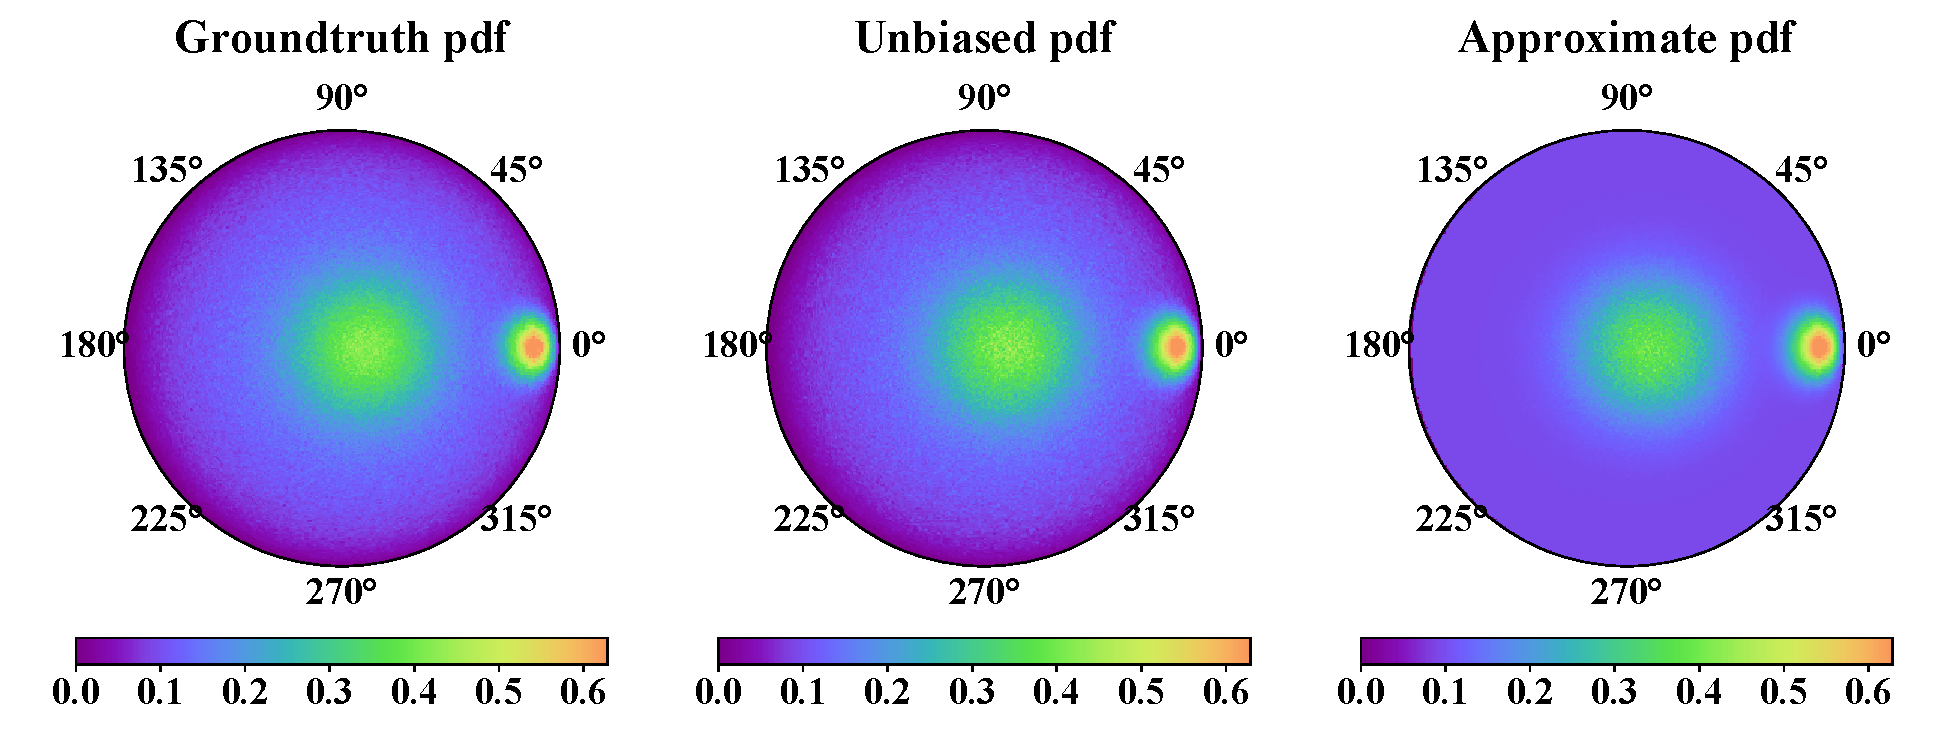
\includegraphics[width=\columnwidth]{img/validations/lobe_pdf/pdf.pdf}
	\caption{\textbf{Validation of our pdf estimates.} The visualization applies a $\log(1+x)$ map for better shape perception. \textbf{Left:} Ground truth by sampling and binning. \textbf{Middle:} Using the unbiased pdf from \S\ref{sssec:ours_pdf_unbiased}. \textbf{Right:} Using the approximate pdf from \S\ref{sssec:ours_pdf_approx} matches the shape of the most important features and approximates longer paths and volume scattering as diffuse.}
	\label{fig:pdf-validate}
\end{figure}




%
\section{Applications and Results}
\label{sec:results}
%
In this section, we \sz{first provide experimental validations (\S\ref{subsec:res_validation})} and then showcase our method on a number of applications and demonstrate its effectiveness (\S\ref{subsec:res_main}).
All the renderings are generated using the Mitsuba physically based renderer~\cite{Mitsuba} with our layered model implemented as a BSDF plugin.
Please see the accompanying video for animated versions of several results.

\sz{
	All the multi-layer results in the paper use our bidirectional estimator with the explicit implementation (although our BSDF plugin also supports nesting BSDFs).
	This is because the former runs faster, as seen in Figure~\ref{fig:result_multilayer}-c.
}
% We currently use double precision floating point arithmetic in all results. 

\sz{

%\vspace{5mm}

\subsection{Validations}
\label{subsec:res_validation}

\subsubsection{Cross validation}
%\myparagraph{Cross validation}
In Figures~\ref{fig:hemispheres} and \ref{fig:pdf-validate} as well as the supplemental material, we cross-validate our Monte Carlo estimators depicted in \S\ref{subsec:ours_eval} by comparing our estimated BSDFs/pdfs to references generated using forward sampling (\S\ref{subsec:ours_sample}) and binning. Notice that the sampling procedure is a straightforward process that requires none of the complexity introduced by our path formulation and estimators.

\subsubsection{White furnace tests}
%\myparagraph{White furnace tests}
We conducted a few ``white furnace tests'' to demonstrate the energy conservation of our layered BSDFs (Figure~\ref{fig:whitetest}).
For all these examples, the BSDFs are constructed such that no energy is lost due to light-layer interactions.
Under constant lighting (where identical amount of light comes from all directions), the object becomes invisible, demonstrating that our layered BSDFs indeed conserve energy properly.
}

% White Furnace test figure
\begin{figure}[h]
	\addtolength{\tabcolsep}{-3.5pt}
	\begin{tabular}{ccc}
		\begin{overpic}[width=0.315\columnwidth]{img/validations/whitetest/sphere_layered_noMedium_env.jpg}
			\put(2,3){\bfseries \color{white} (a1)}
		\end{overpic}
		&
		\begin{overpic}[width=0.315\columnwidth]{img/validations/whitetest/sphere_layered_withMedium_env.jpg} 
			\put(2,3){\bfseries \color{white} (b1)}
		\end{overpic}	
		&
		\begin{overpic}[width=0.315\columnwidth]{img/validations/whitetest/plane_layered_env.jpg} 
			\put(2,3){\bfseries \color{white} (c1)}
		\end{overpic}
		\\
		\begin{overpic}[width=0.315\columnwidth]{img/validations/whitetest/sphere_layered_noMedium_const.jpg}
			\put(2,3){\bfseries (a2)}
		\end{overpic}
		&
		\begin{overpic}[width=0.315\columnwidth]{img/validations/whitetest/sphere_layered_withMedium_const.jpg}
			\put(2,3){\bfseries (b2)}
		\end{overpic}
		&
		\begin{overpic}[width=0.315\columnwidth]{img/validations/whitetest/plane_layered_const.jpg}
			\put(2,3){\bfseries (c2)}
		\end{overpic}
	\end{tabular}
	%
	\caption{\label{fig:whitetest}
		\sz{
			\textbf{White furnace tests.}
			We demonstrate that our BSDFs conserve energy properly via three layered BSDF examples respectively given by
			\textbf{(a)}~a dielectric and a diffuse interface;
			\textbf{(b)}~a dielectric and a conductor interface and participating medium;
			\textbf{(c)}~two dielectric interfaces and participating medium in between.
			All the interfaces and media have albedo one (so no energy is lost due to light-layer interactions).
			For each example, a simple object is rendered under both environmental~(1) and constant~(2) illuminations.
		}
	}
\end{figure}


\subsection{Main Results}
\label{subsec:res_main}

\subsubsection{Application: Coating thickness/normal variation}
%\myparagraph{Application: Coating thickness/normal variation}
%
Figure~\ref{fig:result_glints} shows renderings of a globe with a dielectric coating on top of a metallic substrate.
In this example, both interfaces are colorless and the layer medium has a blue tint.
In Figure~\ref{fig:result_glints}-a, both interfaces are smooth, creating two overlapped reflections of the environment map with different amounts of blur.
In Figure~\ref{fig:result_glints}-b, the top interface of the globe is smooth, leading to one clear reflection.
On the bottom (metallic) interface, we use a detailed height field to drive the normal variation as well as the medium thickness.
The high-frequency variation of normal direction has resulted in detailed highlights on the bottom surface.
Further, due to varying amounts of attenuation at different thickness, these highlights exhibit different colors: reflections from greater depths become darker and more saturated. 
In Figure~\ref{fig:result_glints}-c, the height variation is instead applied to the top dielectric interface, causing the clear reflection of the environment to be replaced by a blurred one.
Further, since the areas under the continents now have larger thickness, their colors become more saturated.
Our layered BSDF model is capable of producing all these appearances using a simple set of parameters (thickness, roughness and medium absorption) in conjunction with spatial variation.

\begin{figure*}[t]
	\centering
	\addtolength{\tabcolsep}{-3pt}
	\begin{tabular}{ccc}
		\begin{overpic}[width=0.32\textwidth]{img/results/glints_globe_none_combine.jpg}
			\put(2,3){\bfseries \large (a)}
		\end{overpic}
		&
		\begin{overpic}[width=0.32\textwidth]{img/results/glints_globe_bottom_combine.jpg}
			\put(2,3){\bfseries \large (b)}
		\end{overpic}
		&
		\begin{overpic}[width=0.32\textwidth]{img/results/glints_globe_top_combine.jpg}
			\put(2,3){\bfseries \large (c)}
		\end{overpic}
	\end{tabular}
	\caption{\label{fig:result_glints}
		\textbf{Top vs. bottom height variation.}
		Thanks to the physically-based nature of our layered BSDF model, manipulating heights on its top and bottom interfaces has greatly varying effects on the final appearance. The height variation drives both normals and thickness differences (and thus medium absorption).
		\textbf{(a)}~No height variation.
		\textbf{(b)}~Height variation applied to the bottom interface.
		\textbf{(c)}~Height variation applied to the top interface.
	}
\end{figure*} 
	

\subsubsection{Application: Complex thin sheet transmission}
%\myparagraph{Application: Complex thin sheet transmission}
%
Our physically based BSDF is capable of accurately modeling not only reflection but also transmission.
Figure~\ref{fig:result_transmit} shows two examples.
The top row contains an example flat surface rendered with our layered BSDF under varying illuminations.
This model involves dielectric interfaces with spatially varying roughnesses and a normal map applied to the front surface.
The optical thickness at each location is obtained by multiplying a base density, which varies across the color channels, by the geometric height field matching the normal map.
In other words, the optical densities (mean free paths) are spectrally varying, which results in subtle color variations across the surface (especially for transmitted light), a phenomenon that would be challenging to model accurately using existing BSDF models. Note again that all of these effects come from the BSDF model, as the scene geometry is a simple flat polygon.

The bottom row of Figure~\ref{fig:result_transmit} shows renderings of a magnifying lens filled with scattering media with spatially varying thickness (which captures the shape of real convex lens). Note that the scene geometry is still just a flat surface.
When coupled with different phase functions (Henyey-Greenstein and von-Mises-Fisher, with different forward scattering parameters), a range of spatially varying and physically plausible blurring effects can be achieved.

Please see the supplemental images and video for more variations with similar configurations.

\begin{figure*}[t]
	\centering
	\addtolength{\tabcolsep}{-3.5pt}
	\begin{tabular}{cccc}
		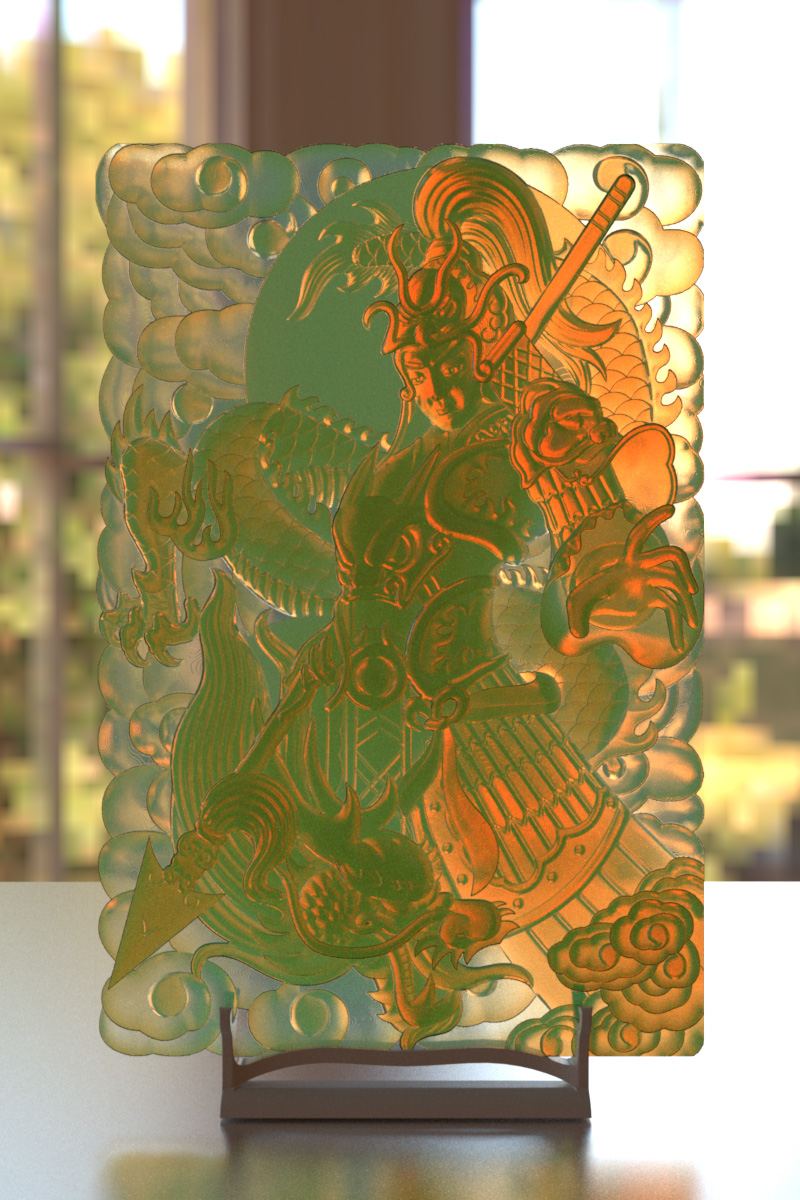
\includegraphics[width=0.24\textwidth]{results/zhaoyun_bg1_1.jpg} &
		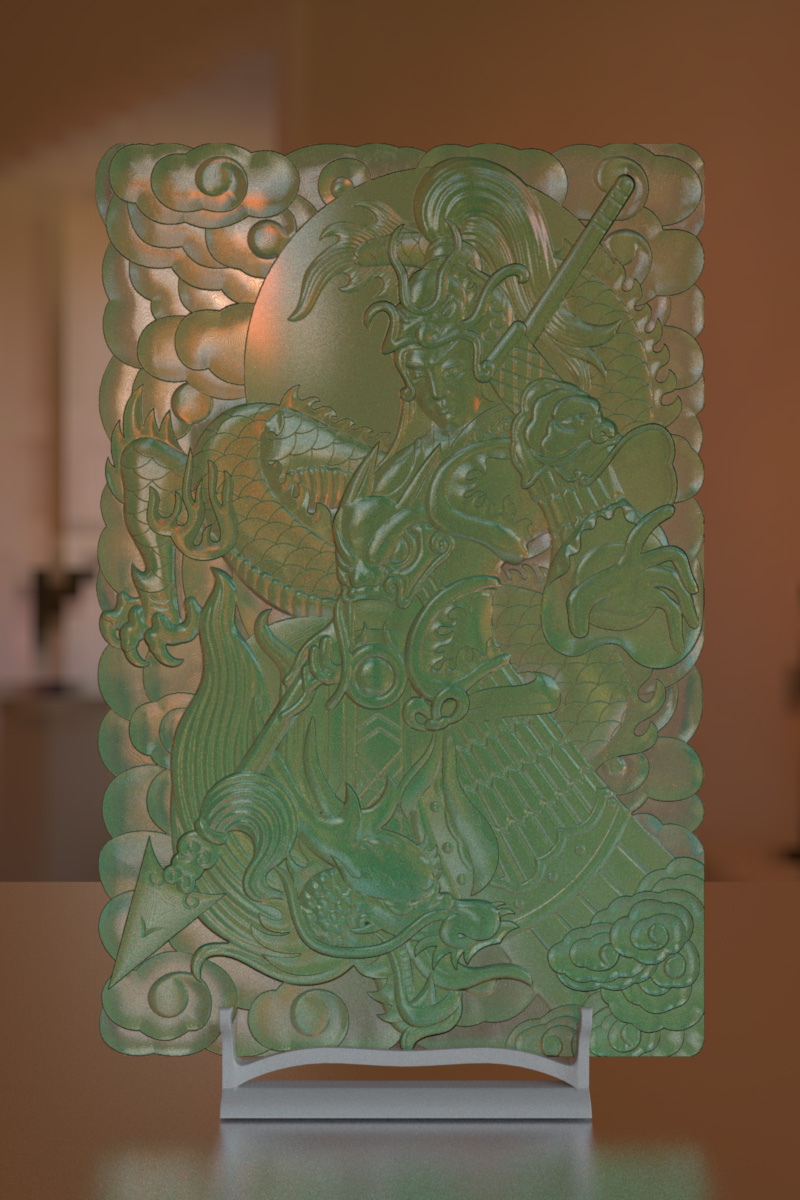
\includegraphics[width=0.24\textwidth]{results/zhaoyun_bg1_2.jpg} &
		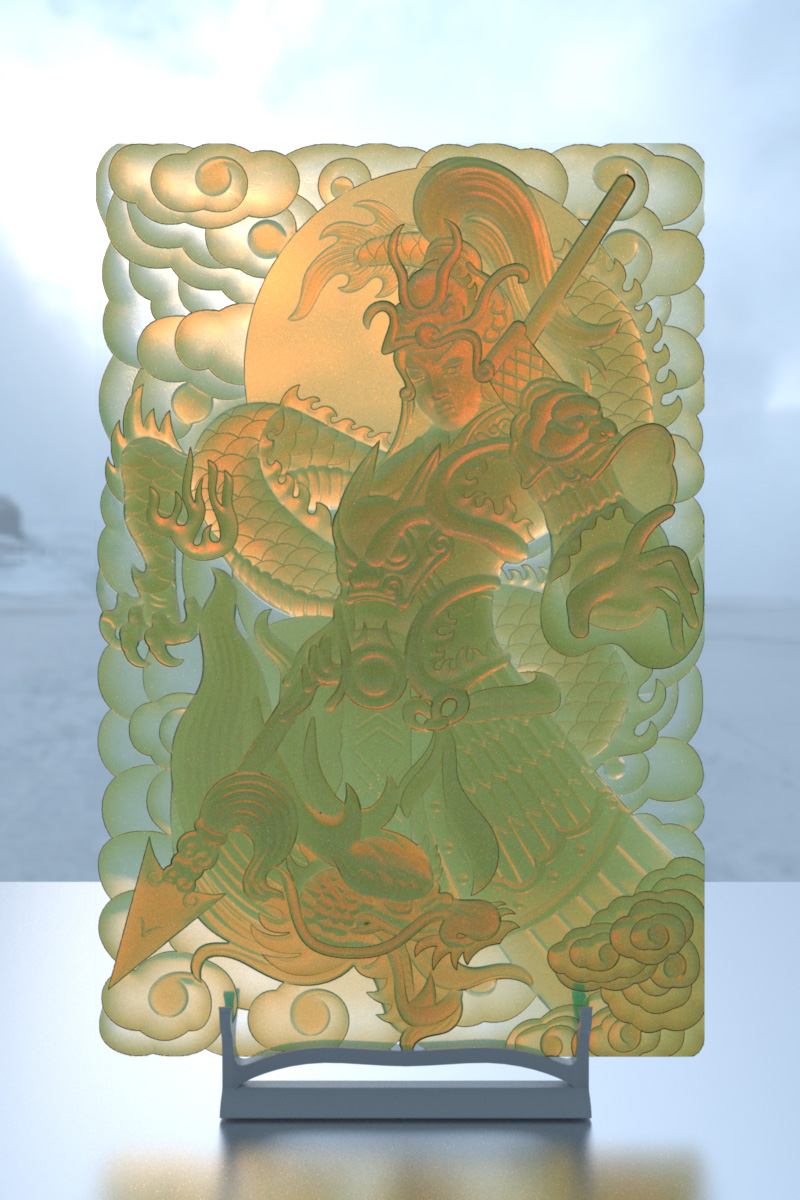
\includegraphics[width=0.24\textwidth]{results/zhaoyun_bg2_1.jpg} &
		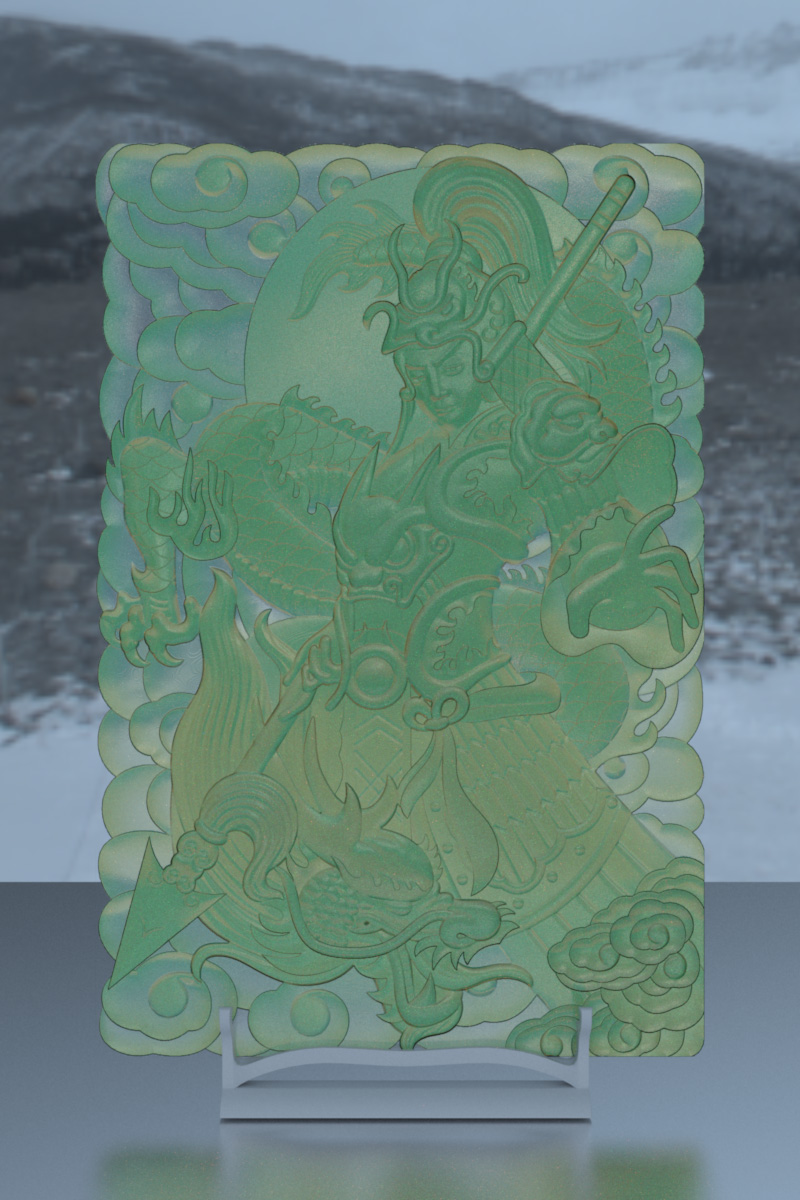
\includegraphics[width=0.24\textwidth]{results/zhaoyun_bg2_2.jpg}\\
		Back-lit & Front-lit & Back-lit & Front-lit
		\\[5pt]
		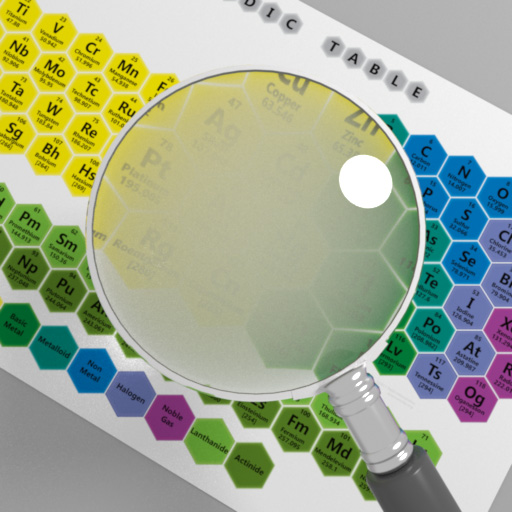
\includegraphics[width=0.24\textwidth]{results/magnify_g9.jpg} &
		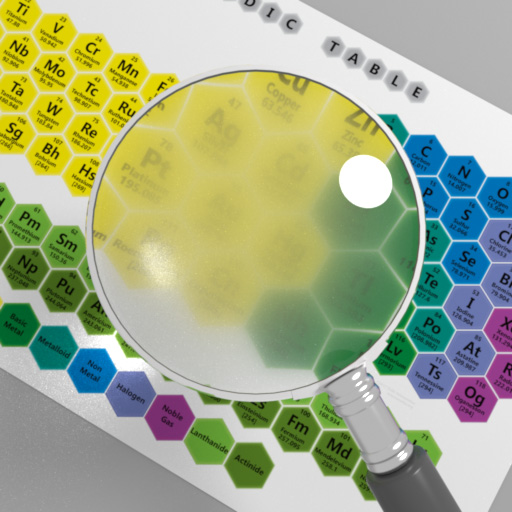
\includegraphics[width=0.24\textwidth]{results/magnify_g99.jpg} &
		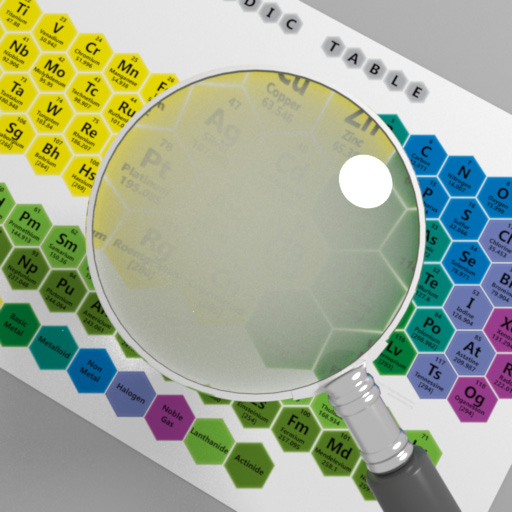
\includegraphics[width=0.24\textwidth]{results/magnify_vmf10.jpg} &
		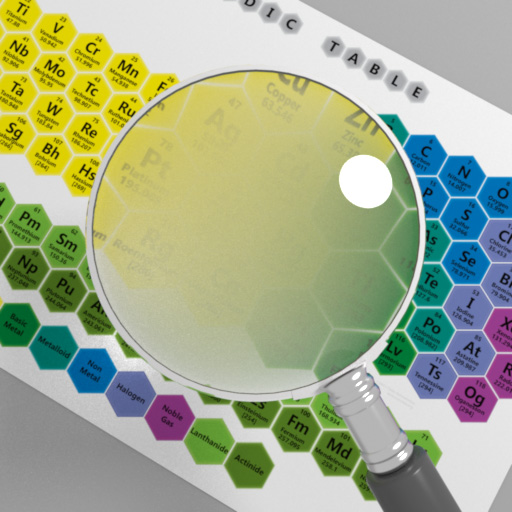
\includegraphics[width=0.24\textwidth]{results/magnify_vmf100.jpg}\\
		HG ($g = 0.9$) & HG ($g = 0.99$) & vMF ($\kappa = 10$) & vMF ($\kappa = 100$)
	\end{tabular}
	%\caption{albedo:0.2,0.95,0.8; $\sigma_t$:1.2,6,12}
	\caption{\label{fig:result_transmit}
		\textbf{Reflection and transmission:}
		Our BSDF models are capable of accurately capturing not only reflection but also transmission from thin layers. \textbf{Top:} A flat surface rendered with our layered BSDF under varying illuminations. This model involves dielectric interfaces with spatially varying roughnesses, normal maps, and thickness. The optical densities (mean free paths) are spectrally varying, which results in subtle color variations across the surface. Note that the color (albedo) is not varying. \textbf{Bottom:} A flat surface with a layered BSDF of spatially varying thickness (which captures the shape of real convex lens). A range of spatially varying and physically plausible blurring effects can be achieved by varying phase functions.
	}
\end{figure*}

\begin{table*}[t]
\centering
	\caption{\label{tab:performance}
		\sz{Render times of all our results (using our ``unidir.'' and ``bidir.'' estimators) as well as baseline models with ``trivial'' BSDFs (that require no stochastic evaluation).
		All the multi-layer models are described using nesting BSDFs for the unidirectional estimator and the explicit implementations for the bidirectional one.
		The baseline models exhibit different appearances and are created solely for performance comparison.
		All the timings are converted to a 6-core Intel i7-6800K CPU time, and those between parentheses indicate render time per mega-pixel.
		The numbers in bold correspond to methods used for creating the paper figures.
		Please refer to the supplemental material for all the other renderings.}
	}
    %
	\begin{tabular}{l|c|c|rr|rr|rr}
	%\hline
	& \multirow{2}{*}{\textbf{Image size}}  & \multirow{2}{*}{\textbf{Spp}} & \multicolumn{6}{c}{\textbf{Render time}}\\
	& & & \multicolumn{2}{c}{\textbf{Unidir.}} & \multicolumn{2}{c}{\textbf{Bidir.}} & \multicolumn{2}{c}{\textbf{Trivial}}\\
	\hline
	\textbf{Fig. \ref{fig:teaser} (a)} & 3000$\times$2000 & 1024           & \sz{2.5 h}  & \sz{(25 m)} & \sz{\textbf{2.2 h}} & \sz{\textbf{(22 m)}}  & \sz{38 m}  & \sz{(6.3 m)}\\
	%\hline
	\textbf{Fig. \ref{fig:result_glints} (b)} & 1024$\times$1024 & 256     & \sz{\textbf{2.2 m}} & \sz{\textbf{(2.1 m)}} & \sz{2.6 m} & \sz{(2.5 m)}   & \sz{1.3 m} & \sz{(1.2 m)}\\
	%\hline
	\textbf{Fig. \ref{fig:result_transmit}, top} & 800$\times$1200  & 512  & \sz{15.2 m}   & \sz{(7.9 m)} & \sz{\textbf{24 m}}  & \sz{\textbf{(12.5 m)}}  & \sz{2.4 m} & \sz{(1.3 m)}\\
	%\hline
	\textbf{Fig. \ref{fig:result_transmit}, bot.} & 512$\times$512   & 1024 & \sz{6.4 m} & \sz{(6.1 m)} & \sz{\textbf{13 m}} & \sz{\textbf{(12.6 m)}}  & \sz{1.6 m} & \sz{(1.5 m)}\\
	%\hline
	\textbf{Fig. \ref{fig:result_mat} (a)} & 876$\times$584   & 256        & \sz{\textbf{1.1 m}} & \sz{\textbf{(2.2 m)}} & \sz{1.4 m} & \sz{(2.7 m)}   & \sz{0.6 m} & \sz{(1.1 m)}\\
	%\hline
	\textbf{Fig. \ref{fig:result_mat} (b)} & 876$\times$584   & 256        & \sz{\textbf{1.1 m}} & \sz{\textbf{(2.2 m)}} & \sz{1.4 m} & \sz{(2.7 m)}   & \sz{0.5 m} & \sz{(0.9 m)}\\
	%\hline
	\textbf{Fig. \ref{fig:result_mat} (c)} & 876$\times$584   & 256        & \sz{\textbf{2.5 m}} & \sz{\textbf{(4.9 m)}} & \sz{5.4 m} & \sz{(10.5 m)}  & \sz{0.5 m} & \sz{(0.9 m)}\\
	%\hline
	\textbf{Fig. \ref{fig:redcloth} (b)} & 640$\times$540   & 256        & \sz{1.5 m}   & \sz{(4.3 m)} & \sz{\textbf{1.9 m}} & \sz{\textbf{(5.5 m)}}   & \sz{0.5 m} & \sz{(1.4 m)}\\
	%\hline
	\textbf{Fig. \ref{fig:result_multilayer} (a)} & 1200$\times$1400 & 256 & \sz{\textbf{6.7 m}}  & \sz{\textbf{(4.0 m)}} & \sz{12 m}  & \sz{(7.1 m)}   & \sz{3.7 m} & \sz{(2.2 m)}\\
	%\hline
	\textbf{Fig. \ref{fig:result_multilayer} (b)} & 1200$\times$1400 & 256 & \sz{\textbf{7.0 m}}  & \sz{\textbf{(4.2 m)}} & \sz{13 m}  & \sz{(7.7 m)}   & \sz{3.7 m} & \sz{(2.2 m)}\\
	%\hline
	\textbf{Fig. \ref{fig:result_multilayer} (c)} & 1200$\times$1400 & 256 & \sz{67 m} & \sz{(40 m)}  & \sz{\textbf{20 m}}  & \sz{(\textbf{12 m})}    & \sz{4.7 m} & \sz{(2.8 m)}\\
	%\hline
	\end{tabular}
	%\\[2pt]
	%\footnotesize{*T/MP: Render time per mega-pixel}
\end{table*}



\subsubsection{Application: Anisotropic layer media for fabrics}
%\myparagraph{Application: Anisotropic layer media for fabrics}
%
Our layered BSDF allows any phase functions within volumetric scattering layers, including anisotropic microflake phase functions~\cite{Jakob:2010:RTF,Zhao:2011:BVA,Heitz:2015:SMD} capable of representing fabrics.
Figure~\ref{fig:result_mat} shows three fabrics modeled using our model with ``null'' top and bottom interfaces (ones that allows light to travel through without reflecting or refracting it) and anisotropic layer media with spatially varying albedo and flake orientations (the optical density does not vary in these examples, though it could).
The satin weave shows well aligned yarns have created smooth and strongly anisotropic highlights. The twill pattern has warp and weft yarns in different colors, leading to dual colored highlights. The velvet exhibits strong grazing-angle highlights, an effect that is challenging to model using traditional BSDF models. Our model successfully captures all the diverse appearances from all three fabrics and produces convincing impressions of these materials.

Figure~\ref{fig:redcloth} shows a fabric rendered using fiber orientation data acquired by micro-CT imaging \cite{Zhao:2011:BVA}. Our rendering uses a fiber orientation map derived from the full data, and matches the full volumetric simulation fairly closely, while being 40 times faster. The speedup is because ours is still a flat BSDF model with parameter mapping, as opposed to full volumetric tracing that requires expensive ray marching through massive data.

\subsubsection{Application: Multiple layers}
%\myparagraph{Application: Multiple layers}
%
Lastly, in Figure~\ref{fig:result_multilayer}, we show rendered results of a kettle with varying layer configurations.
In column~(a), the material has a single transparent water layer with a dielectric interface on the top and a metallic surface on the bottom.
Both interfaces are normal mapped to capture the water drops and the scratches, respectively.
In column~(b), the material shares the same bottom surface as in~(a) but has a smooth top interface and a translucent coating layer with spatially varying optical thickness and albedo, making only part of the bottom surface directly visible.
Lastly, in column~(c), the material has a dual-layer configuration by stacking the layers from~(a) on top of that from~(b).
Our method offers the flexibility to conveniently model all three cases with the last one described using the \sz{explicit implementation} depicted in \S\ref{subsec:multi_layer}.

\subsection{Performance}
%
The Monte Carlo processes for sampling and evaluating our BSDFs do introduce computational overhead.
Table~\ref{tab:performance} lists the performance numbers of all our results.
Further, we provide baseline timings using ``trivial'' BSDFs (that require no stochastic evaluation) to the same scene geometries.
%Without highly scattering medium, rendering with our model is roughly 3$\times$ slower than using standard analytical BSDF models. %(Figure~\todo{XXX}).
Our performance does degrade with the presence of optically thick and highly scattering media.
However, as already demonstrated in Figure~\ref{fig:validation1}, rendering using our model is still significantly faster than explicitly simulating light transport in layered geometries.

\begin{figure*}[t]
	\centering
	\addtolength{\tabcolsep}{-3.5pt}
	\begin{tabular}{ccc}
		\begin{overpic}[width=0.322\textwidth]{img/results/satin_spp128.jpg}
			\put(2,60){\bfseries \color{white} \large (a) Satin}
		\end{overpic}
		&
		\begin{overpic}[width=0.322\textwidth]{img/results/twill_128spp.jpg}
			\put(2,60){\bfseries \color{white} \large (b) Twill}
		\end{overpic}
		&
		\begin{overpic}[width=0.322\textwidth]{img/results/velvet_spp128.jpg}
			\put(2,60){\bfseries \color{white} \large (c) Velvet}
		\end{overpic}
	\end{tabular}
	\caption{\label{fig:result_mat}
		\textbf{Anisotropic media within layers.}
		Our layered BSDF offers the generality to use anisotropic layer media with microflake phase functions.
		This example shows three fabrics modeled with our BSDF model with anisotropic layer media: (a) satin; (b) twill; and (c) velvet.
	}
\end{figure*}    

\begin{figure*}[t]
	\centering
	\addtolength{\tabcolsep}{-3.5pt}
	\begin{tabular}{cccc}
		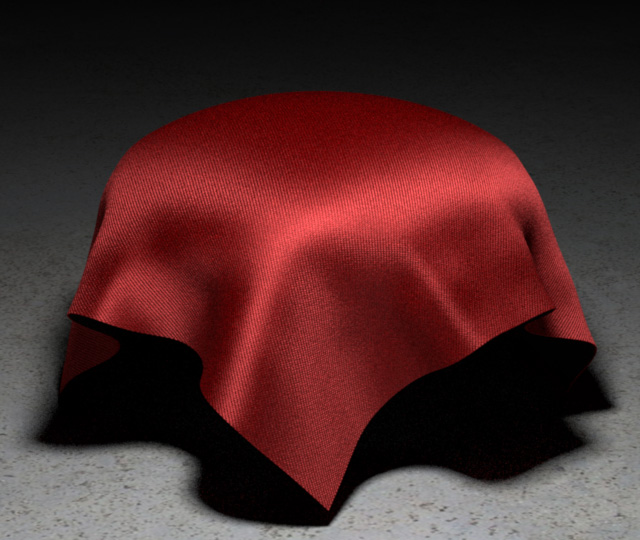
\includegraphics[width=0.24\textwidth]{results/gabardine_ref.jpg} &
		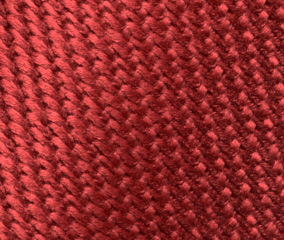
\includegraphics[width=0.24\textwidth]{results/gabardine_ref_inset_128spp.jpg} &
		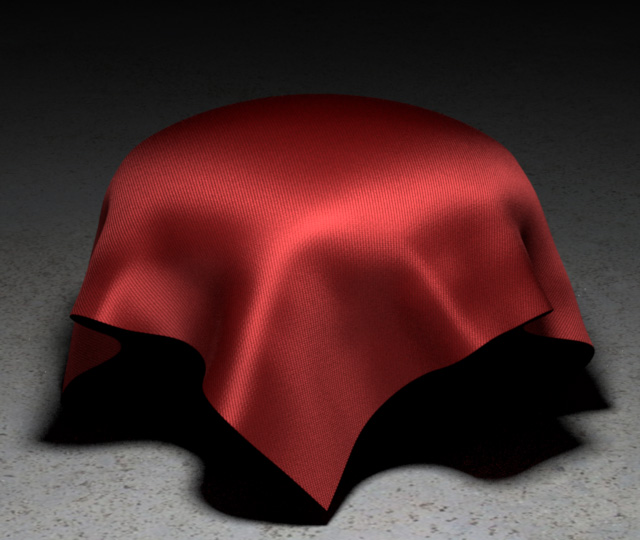
\includegraphics[width=0.24\textwidth]{results/gabardine.jpg} &
		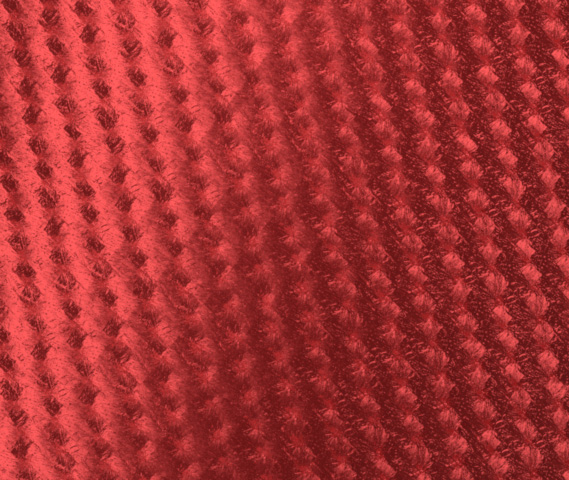
\includegraphics[width=0.24\textwidth]{results/gabardine_inset_512spp.jpg} \\
		\multicolumn{2}{c}{(a) Volume rendering} & \multicolumn{2}{c}{(b) Our BSDF + fiber-direction map}
	\end{tabular}
	\caption{\label{fig:redcloth}
		\textbf{Comparison to volumetric cloth.} \textbf{(a)}~Images rendered from micro-CT volumetric data, using the microflake phase function. \textbf{(b)}~Renderings using our approach using a single microflake volumetric layer, where we are using fiber direction maps extracted from the volumetric data. Our rendering is 40$\times$ faster than the volumetric simulation.
	}
\end{figure*} 


\subsection{Limitations and future work}
\label{subsec:limitation}
%
Our model relies on the assumption of thin flat layers (Figure~\ref{fig:thin_layer}) and cannot capture effects caused by geometric or optical variations at the global scale.
Examples include internal caustics and shadowing arising from major normal variations and color bleeding caused by light scattering though media with varying colors.
Generalizing our technique to include bidirectional subsurface scattering distribution functions (BSSRDFs) is an interesting further topic.
In addition, as our model simulates subsurface scattering using Monte Carlo path tracing, the performance may degrade with the presence of optically thick layers with many scattering events.
Using fast approximated solutions such as~\cite{Jensen:2001:PMS,Frisvad:2014:DDM} to capture multiple scattering may be a useful extension.
Lastly, since we model light transport using traditional radiative transfer, wave effects such as thin film interference are not handled.
An interesting challenge is to integrate wave optics into our model to accurately and efficiently handle light interference and phase shifts.

\begin{figure*}[t]
	\centering
	\addtolength{\tabcolsep}{-3pt}
	\begin{tabular}{ccc}
		\begin{overpic}[width=0.32\textwidth]{img/results/kettle_drop.jpg}
			\put(2,3){\bfseries \color{black} \Large (a)}
		\end{overpic}
		&
		\begin{overpic}[width=0.32\textwidth]{img/results/kettle_logo.jpg}
			\put(2,3){\bfseries \color{black} \Large (b)}
		\end{overpic}
		&
		\begin{overpic}[width=0.32\textwidth]{img/results/kettle_all.jpg}
			\put(2,3){\bfseries \color{black} \Large (c)}
		\end{overpic}
	\end{tabular}
	\caption{\label{fig:result_multilayer}
		\textbf{Multi-layer BSDF.}
		This result shows renderings of a kettle described with: 
		\textbf{(a)}~a single transparent layer with a dielectric top interface capturing the water drops over a conducting bottom surface with scratches; 
		\textbf{(b)}~a single translucent layer with spatially varying optical thicknesses and albedo over the same bottom surface of (a);
		\textbf{(c)}~a dual layer configuration created by stacking the transparent layer~(a) over the translucent one~(b).
	}
\end{figure*}


%
\section{Conclusion}
\label{sec:conclusion}


In this paper, we introduced a new BSDF model to capture the appearance of layered materials. Inside the evaluation and sampling routines of the layered BSDF, we run a Monte Carlo simulation of light transport within flat slabs. This is substantially faster than explicitly constructing the layer geometry, but also allows constructing light transport paths that would not easily be available to a generic light transport algorithm, due to our new position-free path formulation.

Within this framework, we introduced unbiased Monte Carlo techniques analogous to a forward path tracer with next event estimation (NEE) and a fully bidirectional estimator. We demonstrated the capabilities of our solution on a number of examples, featuring multiple layers with surface and volumetric scattering, surface and phase function anisotropy, and spatial variation in all parameters. This leads to the first BSDF layering solution that offers unbiased accuracy and full flexibility in setting the layer properties.


\bibliographystyle{ACM-Reference-Format}
\bibliography{references}

\clearpage
\appendix
\sz{
\section{Detailed Derivations}
\label{sec:derivation}

We now provide detailed derivations for the key equations in \S\ref{sec:path-formulation}.

\myparagraph{Position-free radiative transfer equation}
Traditionally, the radiative transfer equation (RTE) involves an integral over free-flight distance $t$:
%
\begin{multline}
\label{eq:IRTE0}
L_v(z, \bom) = S(z, \bom) \ + \\
\int_0^{t'} \exp(-t \sigma_t) \, \int_{\Sph} \hat f_p(\bom', \bom) \, L_v(z', \bom') \,\intd \bom' \intd t,
\end{multline}
%
where $z' := z - t\cos\bom$ and $t'$ denotes the distance between $z$ and the closest layer boundary.
Since $t = (z - z')/\cos\bom$, changing the integration variable from $t$ to $z'$ in Eq.~\eqref{eq:IRTE0} yields an additional factor of $(\cos\bom)^{-1}$ which in turn gives our position-free RTE~\eqref{eq:IRTE}.
Notice that the change-of-variable ratio only appears within the integration (and not in the source term $S$).

\myparagraph{Cosines in path contribution}
The contribution $f$ of a light path $\bar{x}$ can be obtained by repeatedly expanding the rendering equation~\eqref{eq:RE} and our position-free RTE~\eqref{eq:IRTE}.

Similar to the traditional path integral formulation, for each vertex $z_i$ corresponding to an interface event (i.e., reflection or refraction), a cosine term $|\cos\bd_i|$ is needed to ensure the measure of projected solid angle.
%For the volumetric scattering events, the cosine terms are absent (as the inner integral of the RTE~\eqref{eq:IRTE} already uses the solid angle measure).
On the other hand, a segment of our light path connecting two depths $z_i$ and $z_{i + 1}$ via direction $\bd_i$ can yield an additional $|\cos\bd_i|^{-1}$ when $z_{i + 1}$ corresponds to a volumetric scattering.
Thus, for each $i$, the path contribution involve a factor of $|\cos\bd_i|^{\alpha_i}$ with:
%
\begin{itemize}
	\item $\alpha_i = 1$ if $z_i$ and $z_{i + 1}$ are both on interfaces;
	\item $\alpha_i = 0$ (i.e., no $\cos\bd_i$ term) if (i)~$z_i$ is volumetric and $z_{i + 1}$ lies on an interface (so that no $\cos\bd_i$ terms appear during expansion), or (ii)~$z_i$ is interfacial and $z_{i + 1}$ is volumetric (so that both $|\cos\bd_i|$ and $|\cos\bd_i|^{-1}$ are present, canceling out each other);
	\item $\alpha_i = -1$ if $z_i$ and $z_{i + 1}$ are both volumetric vertices.
\end{itemize}
%
Eq.~\eqref{eqn:seg_contrib_cosine} provides a compact way to encode these rules. 
}

\bigbreak
\section{Efficient Weight Computation}
\label{sec:weight_computation}


\myparagraph{Weights of Light Transport Paths}

Given a light subpath $\bar{x}_i$ and a camera subpath $\bar{x}_o$ with $n_i$ and $n_o$ vertices respectively, our bidirectional estimator combines $2 n_i n_o$ estimators of the form $f(\bar{y}^{(u)}_{s,t})/p^{(u)}_{s,t}(\bar{y}^{(u)}_{s,t})$ with $s \in \{1, 2, \ldots, n_i\}$, $t \in \{1, 2, \ldots, n_o\}$, and $u \in \{0, 1\}$ via the multiple importance sampling (MIS) framework.
This yields a combined estimator:
%
\begin{equation}
\label{eqn:bdpt_estimator}
\sum_{s = 1}^{n_i} \sum_{t = 1}^{n_o} \sum_{u = 0}^1 w^{(u)}_{s, t}(\bar{y}^{(u)}_{s,t}) \frac{f(\bar{y}^{(u)}_{s,t})}{p^{(u)}_{s,t}(\bar{y}^{(u)}_{s,t})},
\end{equation}
%
where the weight $w^{(u)}_{s, t}$, when using the balanced heuristics~[Veach 1997], is given by
%
\begin{equation}
\label{eqn:bdpt_weight_0}
w^{(u)}_{s, t}(\bar{y}_{s,t})
= \left(\sum_{s' = 1}^{s + t - 1} \sum_{u'=0}^1 \frac{p^{(u')}_{s', s + t - s'}(\bar{y}_{s,t})}{p^{(u)}_{s,t}(\bar{y}_{s,t})}\right)^{-1}
\end{equation}
%
for any path $\bar{y}_{s,t}$ with $(s + t)$ vertices.

Notice that, compared to standard bidirectional path tracing that combines $n_i n_o$ estimators, our position-free formulation offers twice the number of estimators since the direction connecting two depths is not unique (see Eq.~(16) of the main paper).


\myparagraph{Efficient Weight Computation}

Computing Eqs.~\eqref{eqn:bdpt_estimator} and \eqref{eqn:bdpt_weight_0} for all $s$ and $t$ na\"ively has a time complexity of $O(n_i n_o (n_i + n_o))$ and is too slow to be practical.
We now present our method that runs in $O(n_i n_o)$ time.
Our approach is conceptually similar to Veach's method for standard BDPT but differs in the exact mathematical form due to our position-free path formulation (see \S4 for the paper).

Let $\bar{y}_{s,t} = (\bd_0, z_1, \bd_1, \ldots, z_n, \bd_n)$ with $n = s + t$.
For all $s', t' \in \{ 1, 2, \ldots, n \}$, define
%
\begin{align}
p^{(0)}_{s'} &:= \prod_{i = 1}^{s' - 1} p( \bd_i \;|\; z_i, \bd_{i - 1} ) \, p( z_{i + 1} \;|\; z_i, \bd_i ),\\
p^{(1)}_{t'} &:= \prod_{i = n - t' + 1}^{n - 1} p( -\bd_i \;|\; z_{i + 1}, -\bd_{i + 1} ) \, p( z_i \;|\; z_{i + 1}, -\bd_i ),
\end{align}
%
which denote the probability for constructing two subpaths containing the first $s'$ and last $t'$ vertices of $\bar{y}$, respectively.
Then, for all $u'$, $s'$ and $t'$, it holds that
%
\begin{equation}
p^{(u')}_{s',t'}(\bar{y}_{s,t}) = p^{(0)}_{s'} \, p^{(1)}_{t'} \, q^{(u')}_{s'},
\end{equation}
%
where
%
\begin{equation}
q^{(u')}_{s'} := \begin{cases}
p( \bd_{s'} \;|\; z_{s'}, \bd_{s' - 1} ) & \text{if $u = 0$,}\\
p( -\bd_{s'} \;|\; z_{s' + 1}, -\bd_{s' + 1} ) & \text{if $u = 1$.}
\end{cases}
\end{equation}
%
It follows that
%
\begin{equation}
\label{eqn:bdpt_pdf_ratio_0}
\frac{p^{(u')}_{s', t'}(\bar{y}_{s,t})}{p^{(u)}_{s,t}(\bar{y}_{s,t})}
= \frac{p^{(0)}_{s'} \, p^{(1)}_{t'} \, q^{(u')}_{s'}}{p^{(0)}_s \, p^{(1)}_t \, q^{(u)}_s}.
\end{equation}
%
Note that, for any $s' < s$, we have
%
\begin{equation}
p^{(u')}_{s', t'}(\bar{y}_{s,t}) = p^{(0)}_{s'} \, \frac{p^{(1)}_{t'}}{p^{(1)}_{t + 1}} \, q^{(u')}_{s'} \,p^{(1)}_{t + 1}.
\end{equation}
%
It follows that
%
\begin{equation}
\label{eqn:bdpt_pdf_ratio_1}
\sum_{s' = 1}^{s - 1} \sum_{u' = 0}^1 \frac{p^{(u')}_{s', t'}(\bar{y}_{s,t})}{p^{(u)}_{s,t}(\bar{y}_{s,t})}
= \frac{p^{(1)}_{t + 1}}{p^{(1)}_t \, q^{(u)}_s}
\underbrace{\sum_{s' = 1}^{s - 1} \sum_{u' = 0}^1 \frac{p^{(0)}_{s'} \frac{p^{(1)}_{t'}}{p^{(1)}_{t + 1}} q^{(u')}_{s'}}{p^{(0)}_s}}_{=:\ P^{(0)}_s}.
\end{equation}
%
Since
%
\begin{equation}
\frac{p^{(1)}_{t'}}{p^{(1)}_{t + 1}}
= \prod_{i = s' + 1}^{s - 1} p( -\bd_i \;|\; z_{i + 1}, -\bd_{i + 1} ) \, p( z_i \;|\; z_{i + 1}, -\bd_i ),
\end{equation}
%
it is easy to verify that $P^{(0)}_s$ depends only on depths $z_{s'}$ and directions $\bd_{s'}$ with $s' \leq s$, which are all from the subpath $\bar{x}_i$.
Further, $P^{(0)}_{s'}$ remains constant for all paths $\bar{y}_{s,t}$ with $s > s'$.
This allows us to precompute $P^{(0)}_s$ using $\bar{x}_i$ for $s = 1, 2, \ldots, n_i$.
To this end, $P^{(0)}_s(\bar{y})$ can be efficiently evaluated using the following relation:
%
\begin{equation}
\label{eqn:bdpt_radio0}
P^{(0)}_s = \begin{cases}
0 & (s = 0),\\
\frac{p^{(0)}_{s - 1}}{p^{(0)}_s} \left( P^{(0)}_{s - 1} \frac{p^{(1)}_{t + 2}}{p^{(1)}_{t + 1}} + \sum_{u'} q^{(u')}_{s - 1} \right) & (s > 1).
\end{cases}
\end{equation}
%
Using Eq.~\eqref{eqn:bdpt_radio0}, we can compute $P^{(0)}_s(\bar{x}_i)$ for $s = 1, 2, \ldots, n_i$ in $O(n_i)$ time.

Similarly, for all $t' < t$, we have
%
\begin{equation}
\label{eqn:bdpt_pdf_ratio_2}
\sum_{t' = 1}^{t - 1} \sum_{u' = 0}^1 \frac{p^{(u')}_{s', t'}(\bar{y}_{s,t})}{p^{(u)}_{s,t}(\bar{y}_{s,t})}
= \frac{p^{(0)}_{s + 1}}{p^{(0)}_s \, q^{(u)}_s}
\underbrace{\sum_{t' = 1}^{t - 1} \sum_{u' = 0}^1 \frac{\frac{p^{(0)}_{s'}}{p^{(0)}_{s + 1}} p^{(1)}_{t'} q^{(u')}_{n - t'}}{p^{(1)}_t}}_{=:\ P^{(1)}_t},
\end{equation}
%
where $P^{(1)}_t$ only depends on $\bar{x}_o$ can be computed in $O(n_o)$ time.

With both $P^{(0)}_s$ and $P^{(1)}_t$ precomputed, Eq.~\eqref{eqn:bdpt_weight_0} becomes
%
\begin{equation}
\small
\label{eqn:bdpt_weight_1}
w^{(u)}_{s, t}(\bar{y}_{s,t})
= \left(1 + P^{(0)}_s + P^{(1)}_t +
\sum_{u'=0}^1 \frac{p^{(u')}_{s - 1, t + 1}(\bar{y}_{s,t}) + p^{(u')}_{s + 1, t - 1}(\bar{y}_{s,t})}{p^{(u)}_{s,t}(\bar{y}_{s,t})}\right)^{-1},
\end{equation}
%
which can be computed in constant time.
This leads to a full bidirectional estimator with time complexity $O(n_i n_o)$.

\bigbreak
\section{MIS with stochastic function and weight evaluation}
\label{sec:weight_computation}

\myparagraph{Introduction}

While Monte	Carlo integration and multiple importance sampling (MIS) are widely used in practice, we use extended versions of these techniques: our MIS weighting is based on approximate (not exact) pdfs, and our weight and function evaluation are both stochastic (i.e. they consume additional random numbers, and are  equal to the true weight and function value only in expectation). For this reason, we review standard Monte Carlo and MIS estimators, and show that our extensions still lead to unbiased results.


\myparagraph{Monte Carlo estimator}

Let $f(x)$ be an integrable function on domain $D$, and let $X$ be a random variable on domain $D$ with probability distribution $p(x)$, such that $p(x) > 0$ whenever $f(x) \neq 0$. An integral

\begin{equation}
I = \int_D f(x) \ dx
\end{equation}

can be approximated by the unbiased estimator

\begin{equation}
X_f = \frac{f(X)}{p(X)}.
\end{equation}

It is easy to see that $X_f$ is an unbiased estimate of $I$:

\begin{equation}
E_X[X_f] = \int_D p(x) \frac{f(x)}{p(x)} \ dx = \int_D f(x) \ dx = I.
\end{equation}

Note, the cancellation of $p(x)$ is always possible due to the assumption that $p(x) > 0$ for all $x$ where $f(x)$ is non-zero.


\myparagraph{Combining estimators through MIS}

Multiple importance sampling (MIS) combines two different sampling strategies (random variables) $X_1$ and $X_2$ on $D$, with pdfs $p_1(x)$ and $p_2(x)$, to compute the integral $I$ more robustly. This is achieved by choosing weighting functions $w_1(x)$ and $w_2(x)$ such that $w_1(x) + w_2(x) = 1$ for all $x \in D$.

Furthermore, we shall require that if $p_1(x) = 0$ or $p_2(x) = 0$, the corresponding $f(x) = 0$.

The integral $I$ is thus split into $I_1$ and $I_2$:

\begin{equation}
I = I_1 + I_2 = \int_D w_1(x) f(x) \ dx + \int_D w_2(x) f(x) \ dx.
\end{equation}

The following are unbiased estimators for $I_1$ and $I_2$:

\begin{equation}
X_f^1 = \frac{w_1(X)f(X)}{p_1(X)} \qquad X_f^2 = \frac{w_2(X)f(X)}{p_2(X)}.
\end{equation}

This can be seen as follows:

\begin{equation}
E_X[X_f^1] = \int_D p_1(x) \frac{w_1(x)f(x)}{p_1(x)} \ dx = \int_D w_1(x) f(x) \ dx = I_1,
\end{equation}

and the same argument works for $I_2$. Again, the reason the cancellation of $p_1(x)$ works is that either it is non-zero, or $f(x) = 0$, due to the assumption above.

Also note that we made no assumptions on the weights other than that they sum to 1. In particular, there is no requirement that the weights be derived from exact pdfs, and we are free to base them on approximate pdfs, among other choices.


\myparagraph{Stochastic function evaluation}

Now suppose that the function evaluation is itself stochastic, i.e. it is an unbiased estimator $f(x,R)$ of the true value of $f(x)$, that uses a uniform random number $R$ on the interval $[0,1)$ during its evaluation. The argument can be easily extended for the case of consuming multiple uniform random numbers. We use a single random number in the proof for brevity.

Because the function estimator is unbiased, we have $E_R[f(x,R)] = \int_0^1 f(x,r) \ dr = f(x)$ for all $x$. Therefore, our full estimator becomes:

\begin{equation}
X_f = \frac{f(X,R)}{p(X)}.
\end{equation}

We can see that this estimator is still unbiased, by computing its expected value over $X$ \emph{and} $R$:

\begin{align}
E_{X,R}[X_f] &= \int_D \int_0^1 p(x) \frac{f(x,r)}{p(x)} \ dr \ dx \nonumber \\
			 &= \int_D p(x) \frac{\int_0^1 f(x,r) \ dr}{p(x)} \ dx \nonumber \\
			 &= \int_D p(x) \frac{f(x)}{p(x)} \ dx = I
\end{align}



\myparagraph{Stochastic weight and function evaluation}

When both the weight evaluation and the function evaluation in an MIS estimator are stochastic, the resulting estimator is still unbiased, provided that the random numbers used by the weight and the function are independent (which enables us to rewrite the joint integral over both random choices into separate integrals). Specifically, consider an unbiased estimator $w_1(x,R_1)$ of the true value of $w_1(x)$, and an unbiased estimator $f(x,R_2)$ of the true value of $f(x)$, based on uniform random numbers $R_1$ and $R_2$ on the interval $[0,1)$. (again, this can be easily extended for the case of consuming multiple uniform random numbers.) The estimator for integral $I_1$ will become:

\begin{equation}
X_f^1 = \frac{w_1(X,R_1) f(X,R_2)}{p_1(X)}
\end{equation}

We can see that this estimator is unbiased, by computing its expected value over $X$, $R_1$ and $R_2$:

\begin{align}
E_{X,R_1,R_2}[X_f^1] &= \int_D \int_0^1 \int_0^1 p_1(x) \frac{w_1(x,r_1) f(x,r_2)}{p_1(x)} \ dr_1 \ dr_2 \ dx \nonumber \\
					 &= \int_D  p_1(x) \frac{\int_0^1 w_1(x,r_1) \ dr_1 \cdot \int_0^1 f(x,r_2) \ dr_2}{p_1(x)} \ dx \nonumber \\
					 &= \int_D  p_1(x) \frac{w_1(x) f(x)}{p_1(x)} \ dx = I_1.
\end{align}

The same argument can be used for $X_f^2$.


\myparagraph{Discussion}

{\bf Application to direct illumination integral.} In our application, the integral of interest $I$ is normally the direct illumination estimate at a shading point. The function $f(x)$ involves the product of the BSDF and illumination values; this is integrated over the unit sphere (or unit hemisphere for BRDFs with no transmission), which is the domain $D$. The random variables $X_1$ and $X_2$ are outgoing directions $\omega_o$ chosen by light sampling and BSDF sampling, respectively. For the case of light sampling, we need to stochastically evaluate the MIS weight and BSDF value for the chosen $\omega_o$; these evaluations will consume vectors of uniform random numbers $R_1$ and $R_2$, respectively.

{\bf No approximation of pdfs in estimator denominators.} While in the main paper we use approximate stochastic pdfs to define the weights, we never approximate the pdfs in the denominators of our estimators. In our case, the accurate values of these pdfs are already baked into the $f/p$ estimates returned by the position-free Monte Carlo simulations.

{\bf Sum of stochastic weights.} The sum of the stochastic approximations to weights $w_1$ and $w_2$ will generally not be exactly 1, but this is not required. We simply require that
\begin{enumerate}
	\item the expected values of the weights sum to 1, so that the integral $I$ separates correctly into $I_1$ and $I_2$,
	\item $X_f^1$ and $X_f^2$ are unbiased estimators for $I_1$ and $I_2$, respectively.
\end{enumerate}
The combination of these properties implies an unbiased estimate for $I$.

\end{document}
